\documentclass[11pt]{article}

% Extract
\usepackage[active,
            generate=topology_definitions,
            %extract-cmd={section},
            extract-env={definition,algorithm}]{extract}

% \usepackage[active,
%             generate=topology_theorems,
%             %extract-cmd={section},
%             extract-env={theorem,corollary,claim}]{extract}

\begin{extract*}

%%%%%%%%%%%%%%%%%%%%%%%%%%%%%%%%%%%%%%%%%%%%%%%%%%%%%%%%%%%%%%%%%%%%%%%%%%%%%%%%%%

% Packages

% AMS 
\usepackage{amsmath, amssymb, amsthm, amsbsy}
% Geometry
\usepackage{geometry}
% Colors
\usepackage[usenames,dvipsnames]{xcolor}
% Figures
\usepackage{graphicx}
\usepackage{float}
% Multi column lists
\usepackage{multicol}
% Subfigures
\usepackage{caption}
\usepackage{subcaption}
% Caligraphic
\usepackage{mathrsfs}
\usepackage{bbm}
% Bold
\usepackage{bm}
% algos
\usepackage[linesnumbered, lined, ruled]{algorithm2e}
% Spacing 
\usepackage{setspace}
% Refs/links
\usepackage[colorlinks=true, citecolor=Blue, linkcolor=blue]{hyperref}
\newcommand\myshade{85}
\colorlet{mylinkcolor}{violet}
\colorlet{mycitecolor}{PineGreen}
\colorlet{myurlcolor}{Aquamarine}

\hypersetup{
  linkcolor  = mylinkcolor!\myshade!black,
  citecolor  = mycitecolor!\myshade!black,
  urlcolor   = myurlcolor!\myshade!black,
  colorlinks = true,
}
% Bibliography
\usepackage{filecontents}
\usepackage{natbib}
% Indent
\usepackage{indentfirst}
% Pretty lists
\usepackage{enumitem}
\setlist[enumerate]{itemsep=2pt,topsep=3pt}
\setlist[itemize]{itemsep=2pt,topsep=3pt}
\setlist[enumerate,1]{label=(\roman*)}

% Code
\usepackage{listings}

% Appendix
\usepackage[toc,page]{appendix}

% Math
\usepackage{mathtools}
\usepackage{xparse}

% Equation numbering
\numberwithin{equation}{section}

% Use more than one optional parameter in a new commands
\usepackage{xargs}                      
% Todo
\usepackage[colorinlistoftodos,prependcaption,textsize=normalsize]{todonotes}
\newcommandx{\unsure}[2][1=]{\todo[linecolor=red,backgroundcolor=red!25,bordercolor=red,#1]{#2}}
\newcommandx{\change}[2][1=]{\todo[linecolor=blue,backgroundcolor=blue!25,bordercolor=blue,#1]{#2}}
\newcommandx{\info}[2][1=]{\todo[linecolor=OliveGreen,backgroundcolor=OliveGreen!25,bordercolor=OliveGreen,#1]{#2}}
\newcommandx{\improvement}[2][1=]{\todo[linecolor=Plum,backgroundcolor=Plum!25,bordercolor=Plum,#1]{#2}}
\newcommandx{\thiswillnotshow}[2][1=]{\todo[disable,#1]{#2}}

% Framed theorems
\usepackage[framemethod=TikZ]{mdframed}

%%%%%%%%%%%%%%%%%%%%%%%%%%%%%%%%%%%%%%%%%%%%%%%%%%%%%%%%%%%%%%%%%%%%%%%%%%%%%%%%%%

% Document Settings

% Figure path
\graphicspath{{./figures/}}
% Matrix columns
\setcounter{MaxMatrixCols}{10}
% So pages will break inside long equation environments
\allowdisplaybreaks
% Font
\usepackage{mathpazo} 
\linespread{1.05}  
%\usepackage{courier}
% Geometry
\geometry{left=1in,right=1in,top=1in,bottom=1in}
% Counters
\setcounter{tocdepth}{2}
\setcounter{secnumdepth}{3}

%%%%%%%%%%%%%%%%%%%%%%%%%%%%%%%%%%%%%%%%%%%%%%%%%%%%%%%%%%%%%%%%%%%%%%%%%%%%%%%%%%

% Colors

\definecolor{Tm}{rgb}{0,0,0.80}
\newcommand{\navy}[1]{\textcolor{MidnightBlue}{\bf #1}}

%%%%%%%%%%%%%%%%%%%%%%%%%%%%%%%%%%%%%%%%%%%%%%%%%%%%%%%%%%%%%%%%%%%%%%%%%%%%%%%%%%


\newcounter{defi}[section]\setcounter{defi}{0}
\newcommand{\thedef}{\arabic{section}.\arabic{defi}}

\newenvironment{defi}[2][]{%
    \refstepcounter{defi}
 
	\ifstrempty{#1}%
	% if condition (without title)
	{\mdfsetup{%
	    frametitle={%
	        \tikz[baseline=(current bounding box.east),outer sep=0pt]
	        \node[anchor=east,rectangle,fill=MidnightBlue!20]
	        {\strut Definition~\thedef};}
	    }%
	% else condition (with title)
	}{\mdfsetup{%
	    frametitle={%
	        \tikz[baseline=(current bounding box.east),outer sep=0pt]
	        \node[anchor=east,rectangle,fill=MidnightBlue!30]
	        {\strut Definition~\thedef:~#1};}%
	    }%
	}%
	% Both conditions
	\mdfsetup{%
	    innertopmargin=10pt,linecolor=MidnightBlue!30,%
	    linewidth=2pt,topline=true,%
	    frametitleaboveskip=\dimexpr-\ht\strutbox\relax%
	}
 
\begin{mdframed}[]\relax}{

\end{mdframed}}


\newcounter{theo}[section]\setcounter{theo}{0}
\renewcommand{\thetheo}{\arabic{section}.\arabic{theo}}

\newenvironment{theo}[2][]{%
    \refstepcounter{theo}
 
	\ifstrempty{#1}%
	% if condition (without title)
	{\mdfsetup{%
	    frametitle={%
	        \tikz[baseline=(current bounding box.east),outer sep=0pt]
	        \node[anchor=east,rectangle,fill=PineGreen!20]
	        {\strut Theorem~\thetheo};}
	    }%
	% else condition (with title)
	}{\mdfsetup{%
	    frametitle={%
	        \tikz[baseline=(current bounding box.east),outer sep=0pt]
	        \node[anchor=east,rectangle,fill=PineGreen!30]
	        {\strut Theorem~\thetheo:~#1};}%
	    }%
	}%
	% Both conditions
	\mdfsetup{%
	    innertopmargin=10pt,linecolor=PineGreen!30,%
	    linewidth=2pt,topline=true,%
	    frametitleaboveskip=\dimexpr-\ht\strutbox\relax%
	}
 
\begin{mdframed}[]\relax}{

\end{mdframed}}


\newcounter{claim}[section]\setcounter{claim}{0}
\renewcommand{\theclaim}{\arabic{section}.\arabic{claim}}

\newenvironment{claim}[2][]{%
    \refstepcounter{claim}
 
	\ifstrempty{#1}%
	% if condition (without title)
	{\mdfsetup{%
	    frametitle={%
	        \tikz[baseline=(current bounding box.east),outer sep=0pt]
	        \node[anchor=east,rectangle,fill=PineGreen!20]
	        {\strut Claim~\theclaim};}
	    }%
	% else condition (with title)
	}{\mdfsetup{%
	    frametitle={%
	        \tikz[baseline=(current bounding box.east),outer sep=0pt]
	        \node[anchor=east,rectangle,fill=PineGreen!30]
	        {\strut Claim~\theclaim:~#1};}%
	    }%
	}%
	% Both conditions
	\mdfsetup{%
	    innertopmargin=10pt,linecolor=PineGreen!30,%
	    linewidth=2pt,topline=true,%
	    frametitleaboveskip=\dimexpr-\ht\strutbox\relax%
	}
 
\begin{mdframed}[]\relax}{

\end{mdframed}}

\newcounter{corollary}[section]\setcounter{corollary}{0}
\newcommand{\thecor}{\arabic{section}.\arabic{corollary}}

\newenvironment{corollary}[2][]{%
    \refstepcounter{corollary}
 
	\ifstrempty{#1}%
	% if condition (without title)
	{\mdfsetup{%
	    frametitle={%
	        \tikz[baseline=(current bounding box.east),outer sep=0pt]
	        \node[anchor=east,rectangle,fill=PineGreen!20]
	        {\strut Corollary~\thecor};}
	    }%
	% else condition (with title)
	}{\mdfsetup{%
	    frametitle={%
	        \tikz[baseline=(current bounding box.east),outer sep=0pt]
	        \node[anchor=east,rectangle,fill=PineGreen!30]
	        {\strut Corollary~\thecor:~#1};}%
	    }%
	}%
	% Both conditions
	\mdfsetup{%
	    innertopmargin=10pt,linecolor=PineGreen!30,%
	    linewidth=2pt,topline=true,%
	    frametitleaboveskip=\dimexpr-\ht\strutbox\relax%
	}
 
\begin{mdframed}[]\relax}{

\end{mdframed}}

\newcounter{lemma}[section]\setcounter{lemma}{0}
\newcommand{\thelem}{\arabic{section}.\arabic{lemma}}

\newenvironment{lemma}[2][]{%
    \refstepcounter{lemma}
 
	\ifstrempty{#1}%
	% if condition (without title)
	{\mdfsetup{%
	    frametitle={%
	        \tikz[baseline=(current bounding box.east),outer sep=0pt]
	        \node[anchor=east,rectangle,fill=PineGreen!20]
	        {\strut Lemma~\thelem};}
	    }%
	% else condition (with title)
	}{\mdfsetup{%
	    frametitle={%
	        \tikz[baseline=(current bounding box.east),outer sep=0pt]
	        \node[anchor=east,rectangle,fill=PineGreen!30]
	        {\strut Lemma~\thelem:~#1};}%
	    }%
	}%
	% Both conditions
	\mdfsetup{%
	    innertopmargin=10pt,linecolor=PineGreen!30,%
	    linewidth=2pt,topline=true,%
	    frametitleaboveskip=\dimexpr-\ht\strutbox\relax%
	}
 
\begin{mdframed}[]\relax}{

\end{mdframed}}

\newcounter{example}[section]\setcounter{example}{0}
\newcommand{\theex}{\arabic{section}.\arabic{example}}

\newenvironment{example}[2][]{%
    \refstepcounter{example}
 
	\ifstrempty{#1}%
	% if condition (without title)
	{\mdfsetup{%
	    frametitle={%
	        \tikz[baseline=(current bounding box.east),outer sep=0pt]
	        \node[anchor=east,rectangle,fill=Aquamarine!20]
	        {\strut Example~\theex};}
	    }%
	% else condition (with title)
	}{\mdfsetup{%
	    frametitle={%
	        \tikz[baseline=(current bounding box.east),outer sep=0pt]
	        \node[anchor=east,rectangle,fill=Aquamarine!30]
	        {\strut Example~\theex:~#1};}%
	    }%
	}%
	% Both conditions
	\mdfsetup{%
	    innertopmargin=10pt,linecolor=Aquamarine!30,%
	    linewidth=2pt,topline=true,%
	    frametitleaboveskip=\dimexpr-\ht\strutbox\relax%
	}
 
\begin{mdframed}[]\relax}{

\end{mdframed}}

\newenvironment{prf}[1][]{%
 
	\ifstrempty{#1}%
	% if condition (without title)
	{\mdfsetup{%
	    frametitle={%
	        \tikz[baseline=(current bounding box.east),outer sep=0pt]
	        \node[anchor=east,rectangle,fill=PineGreen!20]
	        {\strut Proof};}
	    }%
	% else condition (with title)
	}{\mdfsetup{%
	    frametitle={%
	        \tikz[baseline=(current bounding box.east),outer sep=0pt]
	        \node[anchor=east,rectangle,fill=PineGreen!30]
	        {\strut ~#1};}%
	    }%
	}%
	% Both conditions
	\mdfsetup{%
	    innertopmargin=10pt,linecolor=PineGreen!30,%
	    linewidth=2pt,topline=true,%
	    frametitleaboveskip=\dimexpr-\ht\strutbox\relax%
	}
 
\begin{mdframed}[]\relax}{\qed
\end{mdframed}}

% Environments

\theoremstyle{definition}
\newmdtheoremenv{theorem}{\color{ForestGreen}{\textbf{Theorem}}}[section]
% \newtheorem{theorem}{\color{ForestGreen}{\textbf{Theorem}}}[section]
% \newtheorem{claim}{\color{ForestGreen}{\textbf{Claim}}}[section]
% \newtheorem{lemma}[theorem]{\color{ForestGreen}{\textbf{Lemma}}}
% \newtheorem{proposition}[theorem]{\color{ForestGreen}{\textbf{Proposition}}}
% \newtheorem{corollary}[theorem]{\color{ForestGreen}{\textbf{Corollary}}}
% \newmdtheoremenv{lemma}[theorem]{\color{ForestGreen}{\textbf{Lemma}}}
\newmdtheoremenv{proposition}[theorem]{\color{ForestGreen}{\textbf{Proposition}}}
% \newmdtheoremenv{corollary}[theorem]{\color{ForestGreen}{\textbf{Corollary}}}

\newtheorem{axiom}[theorem]{\color{ForestGreen}{\textbf{Axiom}}}
\newtheorem{conjecture}[theorem]{Conjecture}
\newtheorem{case}[theorem]{Case}
\newtheorem{conclusion}[theorem]{Conclusion}
\newtheorem{criterion}[theorem]{Criterion}
\newtheorem{notation}[theorem]{Notation}
\newtheorem{problem}[theorem]{Problem}

\theoremstyle{definition}
% \newtheorem{definition}{\color{MidnightBlue}{\textbf{Definition}}}[section]
\newmdtheoremenv{definition}{\color{MidnightBlue}{\textbf{Definition}}}[section]
% \newtheorem{example}{\color{WildStrawberry}Example}[section]
\newtheorem{assumption}{Assumption}[section]
\newtheorem{condition}[assumption]{Condition}
\newtheorem*{solution}{\color{Goldenrod}Solution}
% \newenvironment{solution}[1][\proofname]{%
%   \proof[\bf \color{Goldenrod}Solution to #1]%
% }{\endproof}

\newtheorem{exercise}{\color{YellowOrange}Exercise}[section]

% Literature Summary Standards
\newtheorem*{motivation}{Motivation}
\newtheorem*{summary}{Summary}
\newtheorem*{remark}{Remark}
\newtheorem*{model}{Model}
\newtheorem*{tresults}{Theoretical Results}
\newtheorem*{eresults}{Empirical Results}

%%%%%%%%%%%%%%%%%%%%%%%%%%%%%%%%%%%%%%%%%%%%%%%%%%%%%%%%%%%%%%%%%%%%%%%%%%%%%%%%%%

% Math macros

% Math ``brackets''
\newcommand\parens[1]{\left( #1 \right)}
\newcommand\squares[1]{\left[ #1 \right]}
\newcommand\braces[1]{\left\{ #1 \right\}}
\newcommand\angles[1]{\left\langle #1 \right\rangle}
\newcommand\ceil[1]{\left\lceil #1 \right\rceil}
\newcommand\floor[1]{\left\lfloor #1 \right\rfloor}
\newcommand\abs[1]{\left| #1 \right|}
\newcommand\dabs[1]{\left\| #1 \right\|}
\newcommand\vect[1]{\mathbf{#1}}
\newcommand\closure[1]{\overline{#1}}
\newcommand\pset[1]{\mathcal{P}\left(#1\right)}
\newcommand\inv[1]{#1^{-1}}
\newcommand\norm[1]{\lVert#1\rVert}

% inner product
\providecommand{\inner}[1]{\left\langle{#1}\right\rangle}
% stochastic dominance
\newcommand{\lesd}{\preceq_{\textrm{SD}}}

% Set builder (use \Set ultimately and separate by ;)
\DeclarePairedDelimiterX{\set}[1]{\{}{\}}{\setargs{#1}}
\NewDocumentCommand{\setargs}{>{\SplitArgument{1}{;}}m}
{\setargsaux#1}
\NewDocumentCommand{\setargsaux}{mm}
{\IfNoValueTF{#2}{#1} {#1\nonscript\:\delimsize\vert\allowbreak\nonscript\:\mathopen{}#2}}%
\def\Set{\set*}%

% Shortcut math
\newcommand{\ls}{\leqslant}
\newcommand{\gs}{\geqslant}
\def\ss{\subset}
\def\sse{\subseteq}
\def\nss{\not \ss}
\def\sps{\supset}
\def\pss{\subsetneq}
\def\prece{\preccurlyeq}
\def\condgap{\hspace{1cm}}
\def\eprec{\preceq}
% argmax and min
\newcommand{\argmax}{\operatornamewithlimits{argmax}}
\newcommand{\argmin}{\operatornamewithlimits{argmin}}
\newcommand{\es}{\emptyset}
% Implication and reverse implication
\def\imp{\Rightarrow}
\def\pmi{\Leftarrow}
% Integers up to number
\newcommand\intsfin[1]{\braces{1, \ldots, #1}}
% Logic
\def\bic{\Leftrightarrow}
% Bold and italic
\newcommand\boldit[1]{\textbf{\textit{#1}}}
% Misc math
\newcommand{\st}{\ensuremath{\ \mathrm{s.t.}\ }}
\newcommand{\setntn}[2]{ \{ #1 : #2 \} }
\newcommand{\cf}[1]{ \lstinline|#1| }
\newcommand{\fore}{\therefore \quad}
\newcommand{\tod}{\stackrel { d } {\to} }
\newcommand{\tow}{\stackrel { w } {\to} }
\newcommand{\toprob}{\stackrel { p } {\to} }
\newcommand{\toms}{\stackrel { ms } {\to} }
\newcommand{\eqdist}{\stackrel{d} {=} }
\newcommand{\iidsim}{\stackrel{\textrm{ {\sc iid }}} {\sim} }
\newcommand{\1}{\mathbbm 1}
\newcommand{\dee}{\,{\rm d}}
\newcommand{\given}{\, | \,}
\newcommand{\la}{\langle}
\newcommand{\ra}{\rangle}

% Shortcut greek
\def\a{\alpha}
\def\b{\beta}
\def\g{\gamma}
\def\D{\Delta}
\def\d{\delta}
\def\z{\zeta}
\def\k{\kappa}
\def\l{\lambda}
\def\n{\nu}
\def\r{\rho}
\def\s{\sigma}
\def\t{\tau}
\def\x{\xi}
\def\w{\omega}
\def\W{\Omega}
% Nice greek
\newcommand{\p}{\varphi}
\newcommand{\e}{\varepsilon}

% Shorcut vectors
\def\vx{\vect{x}}
\def\vy{\vect{y}}
\def\va{\vect{a}}
\def\vb{\vect{b}}

\newcommand{\CC}{\mathbb C}
\newcommand{\FF}{\mathbb F}
\newcommand{\RR}{\mathbb R}
\newcommand{\NN}{\mathbb N}
\newcommand{\PP}{\mathbbm P}
\newcommand{\EE}{\mathbbm E}
\newcommand{\TT}{\mathbbm T}
\newcommand{\VV}{\mathbbm V}
\newcommand{\QQ}{\mathbb Q}
\newcommand{\WW}{\mathbbm W}
\newcommand{\ZZ}{\mathbbm Z}
\newcommand{\UU}{\mathbbm U}
\renewcommand{\SS}{\mathbbm S}

% Expectation/Probability
\newcommand{\ee}[1]{\mathbbm{E}[{#1}]}
\newcommand{\pp}[1]{\mathbbm{P}({#1})}

\newcommand{\GG}{\mathsf G}
\newcommand{\XX}{\mathsf X}
\renewcommand{\AA}{\mathsf A}
\newcommand{\YY}{\mathsf Y}
\newcommand{\ZZZ}{\mathsf Z}

\newcommand{\aA}{\mathscr A}
\newcommand{\iI}{\mathscr I}
\newcommand{\eE}{\mathscr E}
\newcommand{\rR}{\mathscr R}
\newcommand{\lL}{\mathscr L}
\newcommand{\cG}{\mathscr G}

\newcommand{\pP}{\mathcal P}
\newcommand{\aAA}{\mathcal A}
\newcommand{\vV}{\mathcal V}
\newcommand{\mM}{\mathcal M}
\newcommand{\oO}{\mathcal O}
\newcommand{\gG}{\mathcal G}
\newcommand{\hH}{\mathcal H}
\newcommand{\tT}{\mathcal T}
\newcommand{\bB}{\mathcal B}
\newcommand{\zZ}{\mathcal Z}
\newcommand{\cC}{\mathcal C}
\newcommand{\dD}{\mathcal D}
\newcommand{\wW}{\mathcal W}
\newcommand{\uU}{\mathcal U}
\newcommand{\sS}{\mathcal S}
\newcommand{\fF}{\mathcal F}

% Common collections
\def\cA{\col{A}}
\def\cB{\col{B}}
% \def\cC{\col{C}}
\def\cT{\col{T}}
\def\cU{\col{U}}

% Common closures
\def\clA{\closure{A}}
\def\clB{\closure{B}}
\def\clK{\closure{K}}

% operators
\DeclareMathOperator{\cl}{cl}
\DeclareMathOperator{\graph}{graph}
\DeclareMathOperator{\interior}{int}
\DeclareMathOperator{\Prob}{Prob}
\DeclareMathOperator{\determinant}{det}
\DeclareMathOperator{\trace}{trace}
\DeclareMathOperator{\sgn}{sgn}
\DeclareMathOperator{\Span}{span}
\DeclareMathOperator{\diag}{diag}
\DeclareMathOperator{\proj}{proj}
\DeclareMathOperator{\rank}{rank}
\DeclareMathOperator{\cov}{Cov}
\DeclareMathOperator{\corr}{Corr}
\DeclareMathOperator{\var}{Var}
\DeclareMathOperator{\mse}{mse}
\DeclareMathOperator{\se}{se}
\DeclareMathOperator{\row}{row}
\DeclareMathOperator{\col}{col}
\DeclareMathOperator{\range}{rng}
\DeclareMathOperator{\kernel}{ker}
\DeclareMathOperator{\dimension}{dim}
\DeclareMathOperator{\bias}{bias}
\DeclareMathOperator{\dom}{dom}
\DeclareMathOperator{\ran}{ran}
\DeclareMathOperator{\Int}{Int}
\DeclareMathOperator{\Cl}{Cl}
\DeclareMathOperator{\im}{im}

\end{extract*}


\title{Topology Notes}
\author{Rebekah Dix}
\begin{document}
\maketitle
\tableofcontents
\newpage 

\listoftodos
\newpage

\section{Set Theory}

\begin{defi}[Set cardinality $\leq$]{}
	Let $A, B$ be sets. $A$ has \navy{cardinality less than or equal to} $B$ (write $\abs{A} \leq \abs{B}$) if there exists an injection from $A$ to $B$. In notation,
	\begin{equation}
		\abs{A} \leq \abs{B} \iff \exists f:A \to B \text{ injective }
	\end{equation} 
\end{defi}

\begin{theo}[Cantor]{}
	For all sets $X$ (including infinite), $X \not\geq \pP(X)$. That is, there does not exist an injection from $\pP(X)$ to $X$. 
\end{theo}
\begin{prf}
	The proof contains 2 steps:
	\begin{enumerate}
		\item Show that there is no surjection from $X$ to $\pP(X)$. 
		\item Show that (i) implies that there is no injection from $\pP(X)$ to $X$. 
	\end{enumerate}

	We start by proving (ii) through the following lemma:
	\begin{lemma}{}
		Let $C,D$ be sets, $C \neq \emptyset$. If there is an injection $i:C \to D$, then there exists a surjection $j: D \to C$. 
	\end{lemma}
	\begin{prf}
		
	\end{prf}
	The contrapositive of this lemma gives that no surjection from $D \to C$ implies no injection from $C \to D$. 
\end{prf}

\begin{theo}[Informal statement of the axiom of choice]{}
	Given a family $\fF$ of nonempty sets, it is possible to pick out an element from each set in the family. 
\end{theo}

\begin{defi}[Partial order]{}
	A \navy{partial order} is a pair $\aAA = (A, \triangleright)$ where $A \neq \emptyset$ such that  for $a,b,c \in A$
	\begin{enumerate}
		\item Antireflexivity: $a \triangleright a$ never happens.
		\item Transitivity: $a \triangleright b, b \triangleright c \imp a \triangleright c$ 
	\end{enumerate}
\end{defi}
\begin{remark}
	With a partial order, you \emph{can} have incomparable elements. 
\end{remark}

\begin{example}[Partial order]{}
	For any set $X$, a partial order is $(\pP(X), \subsetneq)$. For example, if $X=\Set{1,2}$, then $\Set{1}$ and $\Set{2}$ are incomparable. 
\end{example}

\begin{defi}[Maximal]{}
	Let $(A, \triangleright)$ be a partial order. Then $m \in A$ is maximal if and only if no $a \triangleright m$. 
\end{defi}

\begin{example}[Maximal elements]{}
	The following are examples of posets and their maximal elements: 
	\begin{enumerate}
		\item $(\NN, <)$ has no maximal element (there is no largest natural number).
		\item $(\Set{\Set{1},\Set{2}}, \subsetneq)$ has 2 maximal elements, since the two elements of the set are not comparable. 
	\end{enumerate}
\end{example}

\begin{defi}[Chain]
	A \navy{chain} in a partial order $(A, \triangleright)$ is a $C \subseteq A$ such that $\forall a,b \in C$, $a=b$ or $a \triangleright b$ or $b \triangleright a$. (One interpretation in words, ``$C$ is linear'') 
\end{defi}

\begin{theo}[Zorn's Lemma]{}
	Let $(A, \triangleright)$ be a partial order such that the following condition is satisfied:
	\begin{itemize}
		\item[($\zZ$)] In words, if every chain has an upper bound then there is a maximal element. More precisely, ff $C$ is a chain, then $\exists x$ such that $x \triangle$
	\end{itemize}
\end{theo}

\section{Topological Spaces}

\begin{defi}[Topology, Topological Space]{}
	A \navy{topological space} is a pair $(X,\tT)$ where $X$ is a nonempty set and $\tT$ is a set of subsets of $X$ (called a \navy{topology}) having the following properties:
	\begin{enumerate}
		\item $\emptyset$ and $X$ are in $\tT$.
		\begin{equation}
			\emptyset \in \tT,\ X \in \tT
		\end{equation}
		\item The union of \textit{arbitrarily} many sets in $\tT$ is in $\tT$.
		\begin{equation}
			A_\eta \in \tT \ \forall \eta \in H \imp \bigcup_{\eta \in H} A_\eta = \Set{a \in X \text{ for some (that is, } a \in A_\eta \text{)}} \in \tT
		\end{equation}
		\item The intersection a \textit{finite} number of sets in $\tT$ is in $\tT$.
		\begin{equation}
			A_1, \ldots, A_n \in \tT \imp A_1 \cap \cdots \cap A_n \in \tT
		\end{equation}
	\end{enumerate}
	A set $X$ for which a topology $\tT$ has been specified is called a \navy{topological space}, that is, the pair $(X,\tT)$.
\end{defi}

\begin{example}[Examples of topologies]{}
The following are examples of topologies/topological spaces:
\begin{enumerate}
	\item The collection consisting of $X$ and $\emptyset$ is called the \navy{trivial topology} or \navy{indiscrete topology}. 
	\begin{enumerate}
		\item $\tT = \Set{\emptyset, X}$
	\end{enumerate}
	\item If $X$ is any set, the collection of all subsets of $X$ is a topology on $X$, called the \navy{discrete topology}.
	\begin{enumerate}
		\item $\tT = \pP(X)$
	\end{enumerate}
	\item Let $X = \Set{1}$. Then $\tT = \Set{\emptyset, \Set{1}}$ is a topology.
	\item Sierpinski: Let $X = \Set{a,b}$ and $\tT = \Set{\emptyset, X, \Set{a}}$. In this topology, $b$ is glued to $a$. That is, we can't have a set with $b$ and without $a$. However, $a$ is \emph{not} glued to $a$. 
	\begin{remark}
	Observe that from these examples,
	\begin{equation*}
		\text{indiscrete} \subsetneq \text{Sierpinski} \subsetneq \text{discrete}
	\end{equation*}
	\end{remark}	
	\item $X = \RR$ and $\tT = \Set{\emptyset, X} \cup \Set{[a,\infty); a \in \RR}$.
\end{enumerate}
\end{example}


% \begin{defi}[Open set]
% 	If $X$ is a topological space with topology $\tT$, we say that a subset $U$ of $X$ is an \navy{open set} of $X$ if $U$ belongs to the collection $\tT$.
% \end{defi}

% \begin{defi}[Discrete Topology, Trivial Topology]
% 	If $X$ is any set, the collection of all subsets of $X$ is a topology on $X$, called the \navy{discrete topology}. The collection consisting of $X$ and $\emptyset$ is called the \navy{trivial topology}.
% \end{defi}

% \begin{example}[Finite Complement Topology]
% 	Let $X$ be a set. Let $\tT_f$ be the collection of all subsets of $U$ of $X$ such that $X-U$ is either finite or all of $X$. This is topology. We check the three conditions.
% 	\begin{enumerate}
% 		\item $X \in \tT_f$ since $X - X$ is the empty set, and hence finite. $\emptyset \in \tT_f$ since $X - \emptyset = X$ is all of $X$.
% 		\item Let $\{U_\alpha\}$ be an arbitrary of elements of $\tT_f$. Then
% 		\begin{align*}
% 			X - \bigcup U_\alpha &= X - \left(U_{\alpha_1} \cup \cdots \cup U_{\alpha_n}  \cdots \right) \\
% 			&= (X - U_{\alpha_1}) \cap \cdots \cap (X - U_{\alpha_n}) \cdots \\
% 			&= \bigcap (X - U_\alpha)
% 		\end{align*}
% 		Since each $U_\alpha \in \tT_f$, we know that each $X - U_\alpha$ is finite. The intersection of finite sets is finite, so $\{U_\alpha\} \in \tT_f$. 
% 		\item Let $\{U_i\}$ be a finite collection of sets in $\tT_f$. Then
% 		\begin{align*}
% 			X - \bigcap U_i &= X - \left(U_1 \cap \cdots \cap U_n \right) \\
% 			&= (X - U_1) \cup \cdots \cup (X - U_n) \\
% 			&= \bigcup (X - U_i)
% 		\end{align*}
% 		This is a finite union of finite sets, which is also finite. 
% 	\end{enumerate}
% \end{example}

\begin{defi}[(Strictly) Finer, (Strictly) Coarser, Comparable]{}
	Suppose $\tT$ and $\tT'$ are two topologies on a given set $X$. If $\tT' \supset \tT$, we say that $\tT'$ is \navy{finer} than $\tT$. If $\tT'$ properly contains $\tT$, we say that $\tT'$ is \navy{strictly finer} than $\tT$. For these respective situations, we say that $\tT$ is \navy{coarser} or \navy{strictly coarser} than $\tT'$. We say that $\tT$ is \navy{comparable} with $\tT'$ if either $\tT' \supset \tT$ or $\tT \supset \tT'$.
\end{defi}

\begin{example}[Finest and coarsest topologies]{}
	For any set $X$, the finest topology is the discrete topology and the coarsest topology is the trivial topology. 
\end{example}


\section{Basis for a Topology}

\begin{defi}[Basis, Basis Elements, Topology $\tT$ generated by $\bB$]{}
	If $X$ is a set, a \navy{basis} for a topology on $X$ is a collection $\bB \ss \pP(X)$ of subsets of $X$ (called \navy{basis elements}) such that
	\begin{enumerate}
		\item Every element $x \in X$ belongs to some set in $\bB$. In symbols
		\begin{equation}
			\forall x \in X \ \exists B \in \bB \ s.t. \ x \in B
		\end{equation}
		\item If $x$ belongs to the intersection of two basis elements $B_1$ and $B_2$, then there is a basis element $B_3$ containing $x$ such that $B_3 \subset B_1 \cap B_2$. More generally, in symbols
		\begin{equation}
			\forall B_1,\ldots,B_n \in \bB \ \forall x \in \bigcap_{i=1}^n B_i \ \exists B \in \bB \ s.t. \ x \in B \ss \bigcap_{i=1}^n B_i 
		\end{equation}
	\end{enumerate}
\end{defi}

\begin{example}[Bases]{} The following are example of bases of topologies:
	\begin{enumerate}
		\item $X = \RR$ and $\bB = \Set{(a,b);b>a}$. We can cover $\RR$ with open intervals. Further, a real number $x$ is contained in two intervals $B_1$ and $B_2$, then there will be an open interval $B_3$ contained in the intersection of the two intervals. In this example, we can actually set $B_3 = B_1 \cap B_2$. 
		\item $X = \RR^2$ and $\bB = \Set{\text{interiors of circles}}$. We can cover $\RR^2$ with circles. If $x$ is in the intersection of two circles $B_1$ and $B_2$, then we can construct a circle $B_3$ contained in the intersection $B_1 \cap B_2$. Note in this example, we can just take the actual intersection, as it's not a circle. This example can also be extended to other polygons. 
	\end{enumerate}
\end{example}

\begin{defi}[Topology $\tT$ generated by $\bB$]{}
	If $\bB$ is a basis for a topology on $X$, then we define the \navy{topology $\tT$ generated by $\bB$} as follows: A subset $U$ of $X$ is said to be open in $X$ (that is, to be an element of $\tT$) if for each $x \in U$, there is a basis element $B_x \in \bB$ such that $x \in B_x$ and $B_x \subset U$. Note that each basis element is itself an element of $\tT$. More succinctly:
	\begin{equation*}
		U \ss X: U \in \tT \iff \forall x\in U \ \exists B_x \in \bB \ s.t. \ x \in B_x \ss U
	\end{equation*}
	
\end{defi}

\begin{theo}[Collection $\tT$ generated by a basis $\bB$ is a topology on $X$]{}
\end{theo}
\begin{prf}
	We check the three conditions:
	\begin{enumerate}
		\item The empty set is vacuously open (since it has no elements), so $\emptyset \in \tT$. Further, $X \in \tT$ since for each $x \in X$, there must be at least one basis element $B$ containing $x$, which itself is contained in $X$. 
	\end{enumerate}
	\improvement[inline]{Finish Proof}
\end{prf}

\begin{lemma}[Every open set in $X$ can be expressed as a union of basis elements (not unique)]{}
	Let $X$ be a set and $\bB$ a basis for a topology $\tT$ on $X$. Then $\tT$ equals the collection of all unions of elements of $\bB$. 
\end{lemma}
\begin{prf}
	We need to show two inclusions:
	\begin{enumerate}
		\item Collection of elements of $\bB$ in $\tT$: In the topology $\tT$ generated by $\bB$, each basis element is itself an element of $\tT$. Since $\tT$ is a topology, their union is also in $\tT$. 
		\item Element of $\tT$ in collection of all unions of elements of $\bB$: Take $U \in \tT$. Then we know $\forall x \in U$ $\exists B_x \in \bB$ such that $x \in B_x \in U$. Then we claim that $U = \bigcup_{x \in U} B_x$, so that $U$ equals a union of elements of $\bB$. Indeed, ``$\ss$'' follows since $x \in U \implies x \in B_x$. And, ``$\supset$'' follows since $B_x \ss U$, so that the union of all such $B_x$ is in $U$.  
	\end{enumerate}
\end{prf}

\begin{lemma}[]{}
	Let $(X,\tT)$ be a topological space. Suppose $\cC$ is a collection of open sets of $X$ (i.e., $\cC \ss \tT$) such that for each open set $U$ of $X$ and each $x \in U$ , there is an element $V \in \cC$ such that $x \in V \ss U$. Then $\cC$ is a basis for the topology of $X$ (that is, $\cC$ is a basis \emph{and} $\cC$ generates $\tT$). In notation;
	\begin{equation*}
		\forall U \in \tT \ \forall a\in U \ \exists V \in \cC \ s.t. \ a \in V, V \ss U 
	\end{equation*}
	
\end{lemma}
\begin{prf}
	We first show that $\cC$ is indeed a basis. 

	We then show $\cC$ generates $\tT$. 

	\improvement[inline]{Incomplete.}
\end{prf}


\begin{example}[Countable bases]{}
	Let $X = \RR$ and 
	\begin{itemize}
		\item $\t_1$ is the usual topology.
		\item $\t_2$ is the discrete topology. 
	\end{itemize}

	\begin{claim}{}
		$\t_1$ has a countable basis.
	\end{claim}
	\begin{prf}
		We use the fact that $\QQ$ is countable. We will show that
		\begin{equation}
			\bB = \Set{(a,b); a<b, \ a,b \in \QQ}
		\end{equation}
		generates $\t_1$. Let $U \in \tT$ nonempty and take $a \in U$. Since $U$ is open, there exists an open interval $(c,d)$ with $a \in (c,d) \sse U$. Recall that $\QQ$ is dense in $\RR$. Therefore we can pick rationals $p,q$ with $c<p<a<q<d$. Then $a \in (p,q) \sse (c,d) \sse U$. Therefore $(p,q) \in \bB$ and $\bB$ is a basis for $\t_1$. $\bB$ is countable since $\QQ^2$ is countable. 
	\end{prf}

	\begin{claim}{}
		$\t_2$ doesn't have a countable basis. 
	\end{claim}
	\begin{prf}
		Suppose $\bB$ is a basis for $\t_2$. Let $a \in \RR$. We have that $\Set{a} \in \t_2$. Since $\bB$ generates $\t_2$, there must exist some $U \in \bB$ such that $a \in U \ss \Set{a}$. But then $U = \Set{a}$. Therefore we have found an injection from $\RR \to \bB:a \mapsto \Set{a}$. Therefore $\bB$ is not countable. 
		\improvement[inline]{Clarify.}
	\end{prf}
	
	
	
	
\end{example}


\begin{lemma}[When is one topology finer than another?]{}
	Suppose $\bB$ is a bis s for a topology $\t$ on $X$ and $\bB'$ is a basis for a topology $\t'$ on $X$. The following are equivalent:
	\begin{enumerate}
		\item $\t'$ is finer than $\t$ ($\t' \supset \t$). 
		\item In symbols,
		\begin{equation}
			\forall x\in X \ \forall U \in \t: x \in U \ \exists V \in \t' \ s.t. \ x \in V\sse U
		\end{equation}
		equivalently
		\begin{equation}
			\forall x \in X \ \forall B \in \bB : x \in B \ \exists B' \in \bB' : x \in B' \ss B
		\end{equation}
	\end{enumerate}
\end{lemma}

\begin{defi}[Subbasis]{}
	A \navy{subbasis} for a topology on $X$ is a collection of subsets $\sS \ss \pP(X)$ of $X$ whose union equals $X$ (that is, $\bigcup \sS = X$). The topology generated by the subbasis $\sS$ is defined to be the collection $\tT$ of all unions of finite intersections of elements of $\sS$.
\end{defi}

\section{Continuous Functions}

\begin{defi}[Closed]{}
	A subset $A$ of a topological space $(X,\tT)$ is said to be \navy{closed} if the set $X - A \in \tT$. In words, a subset of a topological space is closed if its complement (in the space) is open. 
\end{defi}

\begin{example}[Sets can be both closed and open]{}
	Let $(X,\tT)$ be a topological space. Then $X - X = \emptyset \in \tT$ and $X - \emptyset = X \in \tT$. Therefore $X, \emptyset$ are both closed and open. We call this type of set \navy{clopen}. Further
	\begin{equation}
		\text{Closed} \neq \text{Not Open}
	\end{equation}
\end{example}

\begin{example}[Sets can be neither closed nor open]{}
	Consider $\QQ$ in the usual topology on $\RR$. 
\end{example}


\begin{defi}[Continuous]{}
	Let $(X,\tT)$ and $(Y,\sigma)$ be topological spaces. A function $f : X \to Y$ is said to be \navy{continuous} with respect to $\tT$ and $\sigma$ if for each open subset $V$ of $Y$, the set $f^{-1}(V)$ is an open subset of $X$. In symbols, $\forall S \in \sigma$, we have that $\inv{f}(S) \in \tT$ (where $\inv{f}(S) = \Set{a \in X; f(a) \in S}$). In words, the preimage of an open set is open. 
\end{defi}

\begin{defi}[Homeomorphic]{}
	The topological spaces $(X,\tT)$ and $(Y,\sigma)$ are \navy{homeomorphic} if there exists a function $f: X \to Y$ such that 
	\begin{enumerate}
		\item $f$ is bijective.
		\item $f$ is continuous.
		\item $\inv{f}$ is also continuous. 
	\end{enumerate}
	We write $(X,\tT) \cong (Y,\sigma)$ or $f: (X,\tT) \cong (Y,\sigma)$. 
\end{defi}
\begin{remark}
	This definition states that we can find a \emph{single} bijection that's continuous in both directions. 
\end{remark}

\begin{example}[Continuous functions]{}
	Let $X$ be a set with more than one element. Let $\tT_{disc} = \pP(X)$ and $\tT_{ind} = \Set{\emptyset, X}$ (that is, the discrete and indiscrete topologies. We require $X$ to have more than one element, else these topologies would be the same). Let $f = id$ (that is $f(x) = x$). Then
	\begin{enumerate}
		\item $f: (X,\tT_{disc}) \to (X,\tT_{ind})$ is \textbf{continuous}. Indeed, if $S \sse X$, $S\in \tT_{ind}$, then $f^{-1}(S) \in \tT_{disc}$, since $\tT_{disc} \supset \tT_{ind}$. 

		\item $f: (X,\tT_{ind}) \to (X,\tT_{disc})$ is \textbf{not continuous}. For example, suppose $X = \Set{1,2}$. Let $S = \Set{1} \in \tT_{disc}$. Then $\inv{f}(\Set{1}) = \Set{1} \not \in \tT_{ind}$. 
	\end{enumerate}
\end{example}

\begin{remark}
	This example motivates a more general claim: Any map into the indiscrete topology or out of the discrete topology is continuous. Further, the identity map from a finer topology to a coarser topology is continuous. 
\end{remark}


\begin{example}[Open, closed, continuous functions]{}
	\begin{defi}[Open map]{}
		$f: (X,\tT) \to (Y,\sigma)$ is an \navy{open map} if $\forall S \in \tT$ we have that $f(S) \in \sigma$ (recall $f(S) = \Set{f(s);s \in S}$). In words: open sets map to open sets. 
	\end{defi}

	\begin{defi}[Closed map]{}
		$f: (X,\tT) \to (Y,\sigma)$ is a \navy{closed map} if $\forall S \ss X$ such that $X - S \in \tT$ we have that $Y - f(S) \in \sigma$. In words: closed sets map to closed sets. 
	\end{defi}
	
	\textbf{Continuous, open, and closed maps don't have clean relationships.} 

	To see this, let $X = \Set{1,2}$.
	\begin{enumerate}
		\item Continuous, not open, not closed map: Let $f : (X,\pP(X)) \to (X,\Set{\emptyset,X})$ be the identity map (discrete to indiscrete). 
		\begin{enumerate}
			\item Continuous: Previous example.
			\item Not open: $\Set{1} \in \pP(X)$ maps to $\Set{1} \not\in \Set{\emptyset,X}$. Thus the map is not open.
			\item Not closed: $X - \Set{1} = \Set{2} \in \pP(X)$, so $\Set{1}$ is closed in $(X,\pP(X))$. But $\{2\} \not\in \Set{\emptyset,X}$. Thus $\Set{1}$ is closed on the left, but not on the right.
		\end{enumerate} 
		\item Open, closed, not continuous map: Let $f : (X,\Set{\emptyset,X}) \to (X,\pP(X))$ be the identity map (indiscrete to discrete).
		\begin{enumerate}
		 	\item Not continuous: Previous example. 
		 	\item Open: Since $\tT_{ind} \ss \tT_{disc}$ 
		 	\item Closed: Since $\tT_{ind} \ss \tT_{disc}$.
		 \end{enumerate} 
		 \item Continuous, closed, not open: Let $X = \RR$ and $\t = \t_e$. Let $Y = \RR^2$ and $\t = \t_{e_2}$ (basis is set of open balls). Define $f: X\to Y: r \mapsto (r,0)$. 
		 \begin{enumerate}
		 	\item Continuous: Clear. 
		 	\item Not open: $\RR$ is sent to the x-axis, which is not open in the plane. 
		 	\item Closed: Fix $A \ss \RR$ closed (in $\t_e$-sense). We need to show that $f(A) = \Set{f(a); a \in A}$ is closed (in $\t_{e_2}$ sense). Thus we must show $\RR^2 - f(A)$ is open, which is equivalent to showing that for all $b \in \RR^2$, there exists an $\e > 0$ such that $B_\e(b) \ss \RR^2 - f(A)$. We prove by cases:
		 	\begin{enumerate}
		 	 	\item $b$ not on x-axis: Let $\e = $ distance from $b$ to x-axis. Thus $B_\e(b) \cap (\text{x-axis}) = \emptyset$, and $f(A) \ss (\text{x-axis})$. Thus $B_\e(A) \cap f(A) = \emptyset$, and $B_\e(b) \ss \RR^2 - f(A)$. 
		 	 	\item $b$ is on x-axis: Look at $a = f^{-1}(b)$ (note: $a$ exists and is unique. $f$ is injective and  hits all of $x$-axis. Thus $b \not\in f(A) \imp a \not\in A $). Since $A$ is closed in $\RR$, if $a \not\in A$, then $\exists \e > 0$ such that $(a-\e,a+\e) \sse \RR - A$. Then 
		 	 	\begin{claim}{}
		 	 		$B_\e(b) \ss \RR^2 - f(A)$
		 	 	\end{claim}
		 	 	\begin{prf}
		 	 		$B_\e(b) \cap (\text{x-axis}) = f((a-\e,a+\e))$. But $f((a-\e,a+\e)) \cap f(A) = \emptyset$, since $(a-\e,a+\e) \cap A = \emptyset$. Thus
		 	 		\begin{align*}
		 	 			B_\e(b) \cap f(A) &= B_\e(b) \cap f(A) \cap (\text{x-axis}) \\
		 	 			&= f((a-\e,a+\e)) \cap f(A) \\
		 	 			&= \emptyset
		 	 		\end{align*}
		 	 		
		 	 	\end{prf}
		 	 	
		 	 \end{enumerate} 
		 \end{enumerate}
	\end{enumerate}
\end{example}

\section{Subspace Topology}

\begin{defi}[Subspace topology]{}
	Given a topological space $(X,\tT)$ and a non-empty set $A \sse X$, the \navy{subspace topology on $A$ induced (or given) by $\tT$} is $(A, \t_A)$ where $\tT_A = \Set{U \cap A; U \in \tT}$. 
\end{defi}

\begin{figure}[H]
	\begin{center}
		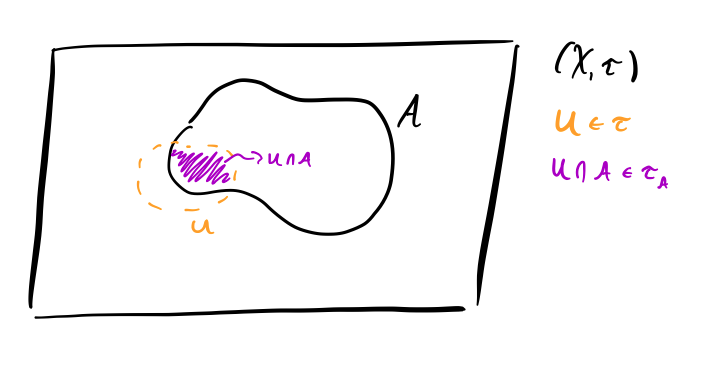
\includegraphics[scale=.4]{subspace_topology.png}
	\end{center}
\end{figure}

\begin{remark}
	Intuitively, $U \cap A$ ``should'' be open in the sense of $A$, since it's the ``all of the open set $U$'' as far as $A$ knows. 
\end{remark}


\begin{prf}[Proof that $(A, \t_A)$ is a topological space]
	We check the axioms:
	\begin{enumerate}
		\item $\emptyset \in \tT_A$: $\emptyset \in \tT$, and $\emptyset \cap A = \emptyset$, so $\emptyset \in \tT_A$. 
		\item $A \in \tT_A$: $X \in \tT$, and $X \cap A = A$, so $A \in \tT_A$.  
		\item Closure under finite intersections [$2$ for simplicity]: Suppose $B_1, B_2 \in \t_A$. We want to show that $B_1 \cap B_2 \in \t_A$. We know that there exist $C_1, C_2 \in \tT$ such that $B_1 = C_1 \cap A$ and $B_2 = C_2 \cap A$. Then
		\begin{equation}
			B_1 \cap B_2 = (C_1 \cap A) \cap (C_2 \cap A) = (C_1 \cap C_2) \cap A
		\end{equation}
		But $C_1 \cap C_2 \in \tT$ since $\tT$ is a topology, therefore $B_1 \cap B_2$ can be written as the intersection of a set in $\tT$ and $A$, so that $B_1 \cap B_2 \in \t_A$. 
	\end{enumerate}
\end{prf}

\begin{claim}[Inclusion is Continuous]{}
	If $(X,\t)$ is a topological space and $A \sse X$, then $f:A \to X:a \mapsto a$ is continuous (with respect to $\t_A$ and $\tau$).
\end{claim}
\begin{prf}
	Let $U \in \t$. Then $\inv{f}(U) = U \cap A$. Therefore $\inv{f}(U) \in \t_A$ by the definition of the subspace topology. 
\end{prf}

\begin{claim}[]{}
	Let $(X,\t)$ and $(Y,\sigma)$ be topological spaces and $f: X\to Y$ be a continuous function (with respect to $\t$ and $\sigma$). Let $A \ss X$ be nonempty and $\t_A$ its subspace topology. Let $B \ss Y$ be nonempty and $\sigma_B$ its subspace topology. Suppose further that $f(A) \sse B$ (that is, for $x \in A$, we have that $f(x) \in B$). Define $\hat f: A\to B: x \mapsto f(x)$ (that is, the restriction of $f$). \textbf{Then} $\hat f: A \to B$ is continuous (with respect to $\t_A$ and $\t_B$). 
\end{claim}
\begin{prf}
	Let $U \ss B$ be $\sigma_B$-open. Then there exists a $W \in \sigma$ such that $U = B \cap W$. Since $f$ is continuous, $\inv{f}(W) \in \t$.  But then $\inv{f}(W) \cap A \in \t_A$ and $\inv{f}(W) \cap A = \inv{f}(U)$. 

	\improvement[inline]{Incomplete}
\end{prf}




\subsection{Connectedness}

\begin{defi}[Connected]{}
	A space $(X,\t)$ is \navy{connected} if whenever sets $V,W$ are
	\begin{enumerate}
		\item Nonempty
		\item Open
		\item $V \cup W = X$
	\end{enumerate}
	we have $V \cap W \neq \emptyset$. 
\end{defi}

\begin{remark}
	Equivalently, a set is connected if and only the only clopen sets are $\emptyset, X$. 
\end{remark}

\begin{example}[Connected Set]{}
	Let $(X,\t) = (\RR,\t_e)$ and $A = (0,1) \cup (1,2)$. Notice that
	\begin{enumerate}
		\item $(0,1) \in \t_A$ since $(0,1) = (0,1) \cap A$ and $(0,1) \in \t_e)$. 
		\item Similarly, $(1,2) \in \t_A$. 
	\end{enumerate}
	Then notice that $(0,1) = A - (1,2)$, so that the complements of both $(0,1)$ and $(1,2)$ are both open. Therefore each set is clopen. Thus $A$ is not connected. 
\end{example}



\section{Metric Spaces}

\begin{defi}[Metric space]{}
	A \navy{metric space} is a nonempty set $X$ together with a binary function $d : X\times X \to \RR$ which satisfies the following properties: For all $x,y,z \in X$ we have that
	\begin{enumerate}
		\item Positivity: $d(x,y) \geq 0$
		\item Definiteness: $d(x,y) = 0$ if and only if $x=y$
		\item Symmetry: $d(x,y) = d(y,x)$
		\item Triangle inequality: $d(x,y) + d(y,z) \geq d(x,z)$
	\end{enumerate}
\end{defi}

\begin{defi}[Metric topology]{}
	Given a metric space $(X,d)$, the set $\bB = \Set{B_\e(x); \e > 0, x \in X}$ is a basis for a topology on $X$ (where $B_\e(x) = \Set{y \in X; d(x,y) < \e}$) called the \navy{metric topology}.
\end{defi}

\begin{defi}[Open Set in Metric Topology]{}
	A set is \navy{open} in the metric topology induced by $d$ if and only if for each $y \in U$ there is a $\d > 0$ such that $B_d(y, \d) \ss U$.
\end{defi}




\begin{theo}[``Continuous'' $=$ ``Continuous'']{}
	If $(X_1,d_1)$ and $(X_2,d_2)$ are metric spaces with induced topologies $\t_{d_1}$ and $\t_{d_2}$, then for $f: X_1 \to X_2$, the following are equivalent:
	\begin{enumerate}
		\item $f$ is continuous with respect to $\t_{d_1}$ and $\t_{d_2}$.
		\item For all $a \in X_1$ and $\e > 0$, there exists a $\d > 0$ such that for all $b \in X_1$ for which $d_1(a,b) < \d$, we have that $d_2(f(a),f(b)) < \e$. 
	\end{enumerate}
\end{theo}
\begin{prf} 
	$(i) \imp (ii)$:
	
	\improvement[inline]{Incomplete.}
\end{prf}

\subsection{Special Properties and Maps}

\begin{defi}[$T_2$, Hausdorff]{}
	$(X,\t)$ is \navy{$T_2$ (Hausdorff)} if for every distinct $a,b \in X$, there exist open sets $V,W \in \t$ such that $a \in V$, $b \in W$, and $V \cap W = \emptyset$.
\end{defi}

\begin{theo}[Separation Axiom]{}
	Metric spaces are always $T_2$. 
\end{theo}
\begin{prf}
	Let $\e = \frac{d(a,b)}{2}$. Then let $V=B_\e(a)$ and $W = B_\e (b)$.
\end{prf}

\begin{remark}
	Not all topological spaces are $T_2$.
\end{remark}

\section{Sequences}

\begin{defi}[Converges]{}
	Fix a topological space $(X,\tT)$. A sequence of points $(a_i)_{i \in \NN} \ss X$ \navy{converges} to $b \in X$ if for every open set $W$ containing $b$, all but finitely many of the terms of the sequence are in $W$. In symbols
	\begin{equation*}
		(a_i)_{i \in \NN} \to b \iff \forall W\in \tT \text{ s.t. } b \in W, \exists N \in \NN \text{ s.t. } \forall m > n, a_m \in W
	\end{equation*}
	
\end{defi}

\begin{defi}[Sequentially closed]{}
	A set $S \ss X$ is \navy{sequentially closed} if for every sequence $(a_i)_{i \in \NN}$ of points in $S$ converging to some $b \in X$, we have $b \in S$. 
\end{defi}

\textbf{How do sequentially closed and closed sets relate?}
\begin{itemize}
	\item In a metric space, a set is closed if and only if it is sequentially closed.
	\item In general topological spaces, this need not be true.
\end{itemize}

\textbf{How bad can convergence be in an arbitrary topological space? Pretty bad.}

\begin{example}[Every sequence converges to every point]{}
	Let $X$ be a set with at least 2 points and $\tT$ be the indiscrete (or trivial) topology (note: $|X| = 1$ isn't that interesting since every sequence in $X$ would then be constant and hence convergent). Let $(a_i)_{i \in \NN}$ be a sequence of points in $X$ and fix a point $b \in X$.

	\begin{claim}[]{}
		$(a_i)_{i \in \NN} \to b$ 
	\end{claim}
	\begin{prf}
		Let $U \ss X$ such that $b \in U$ and $U \in \tT$. Since $b \in U$, we have that $U \neq \emptyset$, so that the only possibility is that $U = X$ (since $\tT = \Set{\emptyset,X}$). But then $U$ contains all elements of the sequence  $(a_i)_{i \in \NN}$. Thus $(a_i)_{i \in \NN}$ converges to $b$. Since $b$ was arbitrary, $(a_i)_{i \in \NN}$ converges to every point of $X$.
	\end{prf}
	
\end{example}

\begin{example}[Every sequence converges to exactly one point or doesn't converge, or converges to everything]{}
	Let $(X,\tT)$ be the cofinite topology (on an infinite set $X$). For simplicity, let $X = \NN$. Let $(a_i)_{i \in \NN}$ be a sequence of points in $X$. We can divide the possible forms of $(a_i)_{i \in \NN}$ into 3 cases:
	\begin{enumerate}
		\item No infinite repetition of any terms (ex. $(1,2,3,4,\ldots)$).
		\item Exactly one value gets repeated infinitely often (ex. $(1,2,1,3,1,4,1,\ldots)$).
		\item At least $2$ values get repeated infinitely often.
	\end{enumerate}
	We will show that the respective outcomes for these cases are
	\begin{enumerate}
		\item Converges to every point.
		\item Converges to point repeated infinitely often.
		\item Doesn't converge.
	\end{enumerate}

	\begin{claim}[]{}
		A sequence with no infinite repetition converges to every point.
	\end{claim}
	\begin{prf}
		 Let $a=(a_i)_{i \in \NN}$ be a sequence in $X$ with no infinite repetition and let $b \in X$. Let $b \in U$ where $U \in \tT$ ($U$ open). Note that $U \neq \emptyset$. Thus $U$ is cofinite (that is, $X-U$ is finite, so that finitely many points of $X$ are \emph{not} in $U$). Therefore each point not in $U$ only appears finitely many times in the sequence (since there is no infinite repetition in $a$). Therefore only finitely many of the terms of $a$ are not in $U$ (finite $\times$ finite = finite). Therefore the sequence converges to $b$. 
	\end{prf}
	
	
\end{example}



\begin{claim}[Metric space: closed $\iff$ sequentially closed]{}
	In a metric space, a set is closed if and only if it is sequentially closed. More formally: If $(X,d)$ is a metric space and $\tT_d$ is the induced topology on $X$, then $S \ss X$ is sequentially closed if and only if $S$ is closed (with respect to $\tT$, that is $X-S \in \tT$). 
\end{claim}
\begin{prf}[Closed $\imp$ sequentially closed]
	Suppose (for contradiction) that $A \ss X$, $A$ closed, but $A$ not sequentially closed. Since $A$ is not sequentially closed, there is a sequence of points  $(a_i)_{i \in \NN}$ from $A$ and a point $b \in X - A$ such that $(a_i)_{i \in \NN} \to b$.  

	$A$ closed means $X- A$ is open. So since $b \in X-A$, there is some $U \in \tT_d$ with $b \in U$ such that $U \cap A = \emptyset$. Of course, $U = X - A$ works. But, we can find a basic open (i.e., a set in the basis we're using, here the set of open balls). Since $b \in X-A$ and $X-A$ open, there exists $\e> 0$ such that $B_\e(b) \ss X-A$. Thus we have that
	\begin{enumerate}
		\item $B_\e(b)$ is open.
		\item $b \in B_\e(b)$.
		\item $B_\e(b)$ contains none of the terms of  $(a_i)_{i \in \NN}$ (since $a_i \in A$ for all $i$). 
	\end{enumerate}
	But then  $(a_i)_{i \in \NN} \not\to b$, a contradiction.
\end{prf}

\section{Product Topology}
\begin{defi}[Product topology, two sets]
	Let $(X,\t)$ and $(Y,\sigma)$ be topological spaces. The \navy{product topology} on $X \times Y$ is the topology having as \emph{basis} the collection $\bB$ of all set of the form $U \times V$ where $U$ is an open subset of $X$ and $V$ is an open subset of $Y$. In symbols,
	\begin{equation}
		\bB_{\t \times \sigma} = \Set{U \times V; U \in \t, V \in \sigma}
	\end{equation}
\end{defi}

\begin{remark}
	Note, open sets of $X \times Y$ need not be of the form open set in X $\times$ open set in $Y$. 
\end{remark}

\begin{prf}[Proof that $\bB_{\t \times \sigma}$ is indeed a basis for a topology on $X \times Y$]
	We check the two conditions required to be a basis:
	\begin{enumerate}
		\item $\bB$ ``covers'' $X$: Note that $X \in \t$ and $Y \in \sigma$ (since they are each topologies). Therefore $X \times Y \in \bB$. Thus for any $(x,y) \in X \times Y$, we have that $(x,y) \in X \times Y \in \bB$.
		\item Intersection Property: Take two basis elements $U_1 \times V_1$ and $U_2 \times V_2$. Notice that
		\begin{equation}
			(U_1 \times V_1) \cap (U_2 \times V_2) = (U_1 \cap U_2) \times (V_1 \cap V_2)
		\end{equation}
		But then $U_1 \cap U_2 \in \t$ and $V_1 \times V_2 \in \sigma$, so that $(U_1 \times V_1) \cap (U_2 \times V_2)  \in\bB$, so the intersection of two basis elements is again a basis element. This is stronger than the property required to be a basis, yet of course sufficient.
	\end{enumerate}
\end{prf}

\begin{defi}[Product space/topology for finitely many spaces]{}
	Let $(X_1,\t_1), \ldots, (X_n,\t_n)$ be topological spaces. The set of points of the \navy{product space} is $X_1 \times \cdots \times X_n$. The basis for the \navy{product topology} is
	\begin{equation}
		\bB_{\t_1 \times \cdots \times \t_n} = \Set{W_1 \times \cdots \times W_n; W_i \in \t_i}
	\end{equation}
\end{defi}

\begin{remark}
	Again, $\bB_{\t_1 \times \cdots \times \t_n}$ is indeed a basis since the first condition is trivially satisfied ($X_1 \times \cdots \times X_n$ is a basis element) and the intersection of products is a product of intersections, and hence again a basis element.
\end{remark}

\begin{defi}[Projection Maps]{}
	Let $(X_1,\t_1)$ and $(X_2,\t_2)$ be topological spaces. Let
	\begin{align*}
		&\pi_1:X_1 \times X_2 \to X_1 : (x_1,x_2) \mapsto x_1 \\
		&\pi_2:X_1 \times X_2 \to X_2 : (x_1,x_2) \mapsto x_2
	\end{align*}
	then $\pi_1$ and $\pi_2$ are \navy{projection maps}. 
\end{defi}

\begin{claim}[]{}
	Let $\pi_1$ be $\pi_2$ projection maps (as above). Then
	\begin{enumerate}
		\item $\pi_1$ is continuous with respect to $\t_1 \otimes \t_2$ and $\t_1$.
		\item $\pi_2$ is continuous with respect to $\t_1 \otimes \t_2$ and $\t_2$.
	\end{enumerate}
\end{claim}
\begin{prf}
	We show $\pi_1$ is continuous. Suppose $S \ss X_1$ is open (i.e., $\in \t_1$). We want to show that $\pi^{-1}(S) \in \t_1 \otimes \t_2$. We have that
	\begin{align*}
		\pi_1^{-1}(S) &= \Set{p \in X_1 \times X_2; \pi_1(p) \in S} \\
		&= \Set{(x_1, x_2) \in X_1 \times X_2; \pi_1((x_1,x_2)) \in S} \\
		&= \Set{(x_1, x_2) \in X_1 \times X_2; x_1 \in S} \\
		&= S \times X_2
	\end{align*}
	Thus we have that
	\begin{itemize}
		\item $S$ is $\t_1$-open.
		\item $X_2$ is $\t_2$-open.
	\end{itemize}
	so that $S \times X_2$ is in our basis for $\t_1 \otimes \t_2$. Thus, $S \times X_2 \in \t_1 \otimes \t_2$.
	
\end{prf}


\begin{example}[Projection Maps]{}
	Take $(X_1,\t_1) = (X_2,\t_2) = (\RR, \t_e)$. Take $S \ss \RR^2$ to be the unit ball: $S = \Set{(x,y);x^2 + y^2 <1}$. Observe that
	\begin{equation}
		\pi_1(S) = \pi_2(S) = (-1,1)
	\end{equation}
\end{example}


\section{Compactness}

\begin{defi}[Open cover]{}
	An \navy{open cover} of $(X,\t)$ is a family of $\t$-open sets $\cC \ss \t$ such that $\bigcup \cC = X$. 
\end{defi}

\begin{remark}
	The notation $\bigcup \cC = X$ means $X$ is the union of ``stuff'' in $\cC$. 
\end{remark}

\begin{example}[Open covers]{}
	The following are examples of open covers of $(X,\t)$:
	\begin{enumerate}
		\item Any basis for $\t$ is an open cover of $(X,\t)$. 
		\item Any subbasis for $\t$ is an open cover of $(X,\t)$.
		\item $\{X\}$.
		\item $\t$.
		\item Let $X = \RR$ and $\t = \t_e$. Then $\uU = \Set{(-n,n); n \in \NN}$ is an open cover of $X$ (call each individual interval $U_n$). (If $\wW \ss \uU$ is finite, let $N = \max\{n : U_n \in \wW\}$. Then $N \not \in \bigcup \wW$)
	\end{enumerate}
\end{example}

\begin{defi}[Subcover]{}
	$\dD$ is a \navy{subcover} of $\cC$ if
	\begin{enumerate}
		\item $\dD \ss \cC$.
		\item $\dD$ is an open cover.  
	\end{enumerate}
	A \navy{finite subcover} is a subcover which is finite.
\end{defi}


\begin{defi}[Compact]{}
	A topological space $(X,\t)$ is \navy{compact} if every open cover has a finite subcover. 
\end{defi}

\begin{example}[Non-compact Set]{}
	Consider the topological space $(\RR,\t_e)$. This space has a finite subcover: $\{\RR\}$. But does this imply that $(\RR,\t_e)$ is compact? No! We need to see if \emph{all} open covers have finite subcovers. Consider the open cover
	\begin{equation}
		\cC = \Set{(-n,n); n \in \NN}
	\end{equation} 
	$\cC$ has no finite subcover. Thus $(\RR,\t_e)$ is not compact. 
\end{example}

\subsection{Applications}

\subsubsection{Optimization}

\improvement[inline]{Incomplete.}

\begin{theo}[Bounded Value Theorem (BVT)]{}
	If $f:[0,1]\to \RR$ is continuous, then $\range{f}$ is bounded (above and below).
\end{theo}

\subsubsection{Cantor Space}

Cantor space $\cC$ has 
\begin{itemize}
	\item Points given by infinite binary sequences (ex.\ $(1,0,1,0,1,0,\ldots)$ is a point). (For concreteness, can think about base-2 representation of numbers in $[0,1]$).
	\item Open sets are generated by finite strings: $U \ss \cC$ is open if and only if for all $f \in U$, there exists a finite binary string $\sigma$ such that every infinite binary sequence beginning with $\sigma$ is in $U$.   
\end{itemize}

\begin{theo}[]{}
	The Cantor Space $\cC$ is compact. 
\end{theo}
\begin{prf}
	
\end{prf}



\improvement[inline]{Incomplete.}

\subsection{Creating New Compact Spaces from Old}

\begin{theo}[``Continuous images'' of compact spaces are compact]{}
	Suppose $(X,\t)$ is compact and $f:(X,\t) \to (Y,\sigma)$ is continuous and surjective (that is, $Y = \im f$). Then $(Y,\sigma)$ is compact. 
\end{theo}
\begin{prf}
	Let $\uU$ be an open cover of $Y$. We must show there exists a finite subcover. For $U \in \uU$ Let $W_U = \inv{f}(U)$. $W_U$ is open since $f$ is continuous and $U \in \sigma$ (open in $Y$). Then $\Set{W_U: U \in \uU}$ covers $X$. To see this, take $x \in X$. Then $f(x) \in Y$, so that there exists some $U \in \uU$ containing $f(x)$. But then $x \in \inv{f}(U) = W_u$. $(X,\t)$ is compact, so $\Set{W_U: U \in \uU}$ has a finite subcover: $\Set{W_{U_i}}_{i=1}^n$. $f$ is surjective, so 
	\begin{equation}
		\bigcup_{i=1}^n f(W_{U_i}) = \bigcup_{i=1}^n U_i = Y
	\end{equation}
	is a finite subcover of $Y$. 

	\textbf{Proof summary:} ``Pull back (continuity), push forward (surjectivity).''
\end{prf}

\begin{corollary}{}
	$[0,1]$ is compact. 
\end{corollary}
\begin{prf}
	Use the map from cantor space $\cC$ to $[0,1]$ that is the binary expansion. That is, $\cC \to [0,1] : f \mapsto f(1)f(2)f(2)\ldots$ in binary. This is a continuous surjection, and $\cC$ is compact, so that by the above theorem, $[0,1]$ is compact. 
\end{prf}



\begin{theo}[Closed subspaces of compact spaces are compact]{}
	If $(X,\t)$ is compact and $A \sse X$ is closed, then $(A,\t_A)$ is compact. 
\end{theo}
\begin{prf}
	Let $\uU$ be an open cover of $A$. Using the definition of the subspace topology, we can write each $U \in \uU$ as $U = V_U \cap A$ where $V_U \in \t$. Since $A$ is closed, we have that $X-A$. Therefore we can form an open cover of $X$ by
	\begin{equation}
		\hat\uU = \Set{V_U: U \in \uU} \cup \Set{X-A}
	\end{equation}
	$\hat\uU$ must have a finite subcover since $X$ is compact, and therefore this finite subcover must use finitely many elements from the set $\Set{V_U: U \in \uU}$ (say $V_{U_1},\ldots, V_{U_n})$. But then
	\begin{equation}
		A \sse \bigcup_{i=1}^n U_i
	\end{equation}
	is a finite subcover of $A$. Therefore every open cover of $A$ has a finite subcover, so $A$ is compact. 
\end{prf}

\begin{theo}[Finite Tychonoff]{}
	Suppose $(X,\t)$ and $(Y,\sigma)$ are compact spaces. Then their product $(X\times Y, \t \otimes \sigma)$ is compact. This also holds for $n$ spaces with $n < \infty$. 
\end{theo}
\begin{prf}
	We prove the case of $n=2$.
	\improvement[inline]{Incomplete.}
\end{prf}

\begin{example}[Example of Finite Tychonoff]{}
	The closed unit cube $[0,1]\times[0,1] \times [0,1]$ is compact. 
\end{example}

\subsection{Tychonoff's Theorem}

\begin{defi}[Cartesian Product (Possibly Infinite)]{}
	Let $\Set{X_i}_{i\in I}$ be a family of sets, where $I$ is an arbitrary index set. The \navy{Cartesian product} $\prod_{i \in I} X_i$ is the set of all functions $f$ such that
	\begin{enumerate}
		\item $f: I \to \cup_{i \in I} X_i$ 
		\item $f(i) \in X_i$
	\end{enumerate}
	In words, $f$ picks out a point from each set. In notation
	\begin{equation}
		\prod_{i \in I} X_i = \Set{f: I \to \cup_{i \in I} X_i; f(i) \in X_i) \forall i \in I}
	\end{equation}
\end{defi}

\improvement[inline]{Figure.}

\begin{example}[Finite Cartesian Product]{}
	Let's check that this definition agrees with the standard notion of a finite Cartesian product. 

	Let $I = \Set{1,2}$. The point $p = (a,b) \in X_1 \times X_2$ corresponds to the function
	\begin{equation}
		f: \Set{1,2} \to X_1 \cup X_2 : 
		\small
		\begin{array}{l}
		1 \mapsto a \quad \text{(1st coordinate of $p$ is $a$)}\\
		2 \mapsto b \quad \text{(2nd coordinate of $p$ is $b$)}\\
		\end{array}
		\normalsize
	\end{equation}
\end{example}

\begin{defi}[Product Space]{}
	Let $I$ be an arbitrary index set. Suppose for each $i \in I$ we have that $(X_i, \t_i)$ is a topological space. Their \navy{product space} has
	\begin{itemize}
		\item Underlying set:
		\begin{equation}
			\prod_{i \in I} X_i
		\end{equation}
		\item Topology: 
		\begin{itemize}
			\item Informally: $\bigotimes_{i \in I} \t_i$ generated by the subbasis of ``wedges'': that is, the topology generated by the subbasis
			\begin{equation}
				\bB = \text{``all sets of the form''} \quad \cdots \times X_i \times X_j \times \cdots \times \underbrace{U}_{n \text{th term}} \times X_k \times \cdots  	
			\end{equation} 
			for $U$ open in $\t_n$.
			\improvement[inline]{Figure.}
			\item Formally: $\bigotimes_{i \in I} \t_i$ generated by the subbasis $\bB$, which is sets of the form 
			\begin{equation}
				\Set{f \in \prod_{i \in I} X_i; f(k) \in W} \quad k \in I, W \in \t_k
			\end{equation}
			\item Alternative: $\bigotimes_{i \in I} \t_i$ is the coarsest topology making all projection maps continuous (where $\pi_i: f \mapsto f(i)$).
			\begin{equation}
				\pi_i^{-1}(U) \in \bB
			\end{equation}
			\improvement[inline]{What does this mean?}
		\end{itemize}
	\end{itemize}
\end{defi}

\begin{theo}[Full Tychonoff]{}
	Suppose $(X_i,\t_i)$ is compact for all $i \in I$. Then the space 
	\begin{equation}
		\parens{\prod_{i \in I} X_i, \bigotimes_{i \in I} \t_i}
	\end{equation}
	is compact. 
\end{theo}

\subsubsection{Ultrafilters}

\begin{defi}[Ultrafilter]{}
	Suppose $I$ is an set (wlog infinite). An \navy{ultrafilter $\UU$} on $I$ is a family of subsets of $I$ such that:
	$\UU$ is a filter:
	\begin{enumerate}
		\item \textbf{Contains $I$, not $\emptyset$}: $I \in \UU$, $\emptyset \not\in \UU$.
		\item \textbf{Closed upwards}: $A \in \UU, \ A \sse B \imp B \in \UU$.
		\item \textbf{Closed under finite intersections:} $A_1, \ldots, A_n \in \UU \imp A_1 \cap \cdots \cap A_n \in \UU$. 
	\end{enumerate}
	and $\UU$ satisfies the additional ``ultra'' condition:
	\begin{enumerate}
		\item[(iv)] $\forall A \sse I$, $A \in \UU$ or $I - A \in \UU$ (but not both, by (i) and (iii))
	\end{enumerate}
\end{defi}

\begin{example}[Frechet Filter]{}
	Recall that a set is cofinite if its complement is finite. 
	Then
	\begin{equation}
		\fF = \Set{\text{cofinite subsets of $I$}} 
	\end{equation}
	is a filter on $I$. Note that
	\begin{itemize}
		\item Each cofinite set is ``most'' of $I$
		\item This is not a topology (doesn't have $\emptyset$)
	\end{itemize}
	We check the conditions required to be a filter:
	\begin{enumerate}
		\item $I - I = \emptyset$, which is finite, so $I \in \fF$. 

		$I - \emptyset = I$, which is assumed infinite, so $\emptyset \not\in \fF$. 
		\item Let $A \in \fF$ and $B \sse I$ such that $A \sse B$. Then $I - B \sse I - A$, and $I - A$ is finite, so $I - B$ must be finite. Therefore $B \in \UU$. 
		\item (For simplicity, check with two sets) Let $A_1, A_2 \in \UU$. Then 
		\begin{equation}
		 	I - (A_1 \cap A_2) = (I - A_1) \cup (I - A_2)
		\end{equation} 
		Each of $(I - A_1)$ and $(I - A_2)$ is finite, so that their union is also finite. Therefore $A_1 \cap A_2 \in \UU$. 
	\end{enumerate}
\end{example}

\begin{example}[Principal filter]{}
	Suppose $I = \NN$. The set
	\begin{equation}
		\fF = \Set{\text{all sets containing } 7}
	\end{equation}
	is a filter. Note:
	\begin{itemize}
		\item We can interpret this filter like a dictatorship in voting.
		\improvement[inline]{Complete intuition.}
	\end{itemize}
	We check the conditions:
	\begin{enumerate}
		\item $12 \in \NN$, so $I = \NN \in \fF$.

		$12 \not\in \emptyset$, so $\emptyset \not\in\fF$. 
		\item Clear.
		\item Clear. 
	\end{enumerate}
\end{example}

\begin{defi}[Principal ultrafilter]
	\navy{Principal ultrafilters} take the form
	\begin{equation}
		\angles{a} = \Set{A \sse I: a \in A} \qquad \text{ for some } a \in I
	\end{equation}
\end{defi}


\begin{example}[Frechet filter is not an ultrafilter]{}
	For a concrete example, let $I = \NN$, $A = \Set{\text{evens}} \ss I$. But $A \not\in \UU$ and $I-A\not\in\UU$.  
\end{example}

\begin{example}[Principal filters are ultrafilters]{}
	Consider $I = \NN$. Let $A \sse \NN$. Then $7 \in A$ or $7 \in \NN - A$. 
\end{example}

\begin{example}[Interpretation of non-principal ultrafilter]{}
	Think of a game of $\infty$-questions. The premise of the game: I have $n \in \NN$, and you want to find it. Example questions:
	\begin{center}
		\begin{tabular}{l|l}
			Q & A \\
			\hline 
			Even & No \\
			$> 3$ & Yes \\
			Prime & No \\
			$> 500$ & Yes \\
			Div 13 & No
		\end{tabular}
	\end{center}
	A non-principal ultrafilter is a cheating strategy where you never get caught (all my answers are consistent). The strategy is: 
	\begin{align*}
		Q &: \text{``Is $n \in A$''} \\
		A &:
		\begin{cases}
			A \in \UU & \text{yes} \\
			\NN - A \in \UU & \text{no}
		\end{cases}
	\end{align*}

	This is an ultrafilter:
	\begin{enumerate}
		\item The number needs to be in $\NN$. 
		\item We need closure upwards (so we don't get caught with a finite set of consistent answers remaining).
		\item We need to answer compound questions correctly. 
	\end{enumerate}

	This ultrafilter is non-principal: We never say yes to a specific number. 
\end{example}

\begin{defi}[Finite intersection property (FIP)]{}
	A collection of subsets $\fF$ of $I$ has \navy{FIP} if whenever $A_1,\ldots,A_n \in \fF$ we have $\bigcap_{i=1}^n A_i \neq \emptyset$. 
\end{defi}

\begin{corollary}{}
	There exist non-principal ultrafilers. 
\end{corollary}
\begin{prf}
	Let $I$ be an infinite set and let $\fF$ be the Frechet filter on $I$. Filters have FIP by properties (i) (contains the entire set and \emph{doesn't} contain the empty set) and (iii) (closed under finite intersections). Indeed, since the finite intersection of any elements of $\fF$ must be in $\fF$, and the empty set is not in $\fF$, filters have FIP. By Theorem \ref{thm:fipextension}, there exists an ultrafilter $\UU$ such that $\UU \supseteq \fF$. 

	\begin{claim}{}
		$\UU$ is non-principal. 
	\end{claim}
	\begin{prf}
		Suppose that $\UU$ were principal. Then by definition $\Set{a} \in \UU$ for some $a \in I$. But $I - \Set{a}$ is cofinite. Therefore $I - \Set{a} \in \fF \sse \UU$. This already contradicts property (iv) (the ultra condition). We also have a contradiction to (i) (doesn't contain the empty set). Indeed, $(I - \Set{a}) \cap \Set{a} = \emptyset \in \UU$, since $\UU$ is closed under finite intersections. 
	\end{prf}
	
	Therefore, extending the Frechet filter gives us a non-principal ultrafilter. 
\end{prf}

\begin{theo}[FIP $\imp$ ultrafilter extension]{}\label{thm:fipextension}
	If $\fF$ has FIP, then there exists an ultrafilter $\UU$ extending $\fF$. That is, $\exists \UU$ such that $\UU \supseteq \fF$. 
\end{theo}
\begin{prf}
	Define a partial order as follows: let \[\PP = \Set{ \text{ set of subsets of I which (i) have FIP and (ii) are supersets of $\fF$}}\] 
	Formally
	\begin{equation}
		\PP = \Set{A \sse \pP(I); A \supseteq \fF \text{ and $A$ has FIP}}
	\end{equation}
	The partial order $\triangleleft$ is $\subsetneq$. 

	\begin{example}[]{}
		Even/Odd

		\improvement[inline]{Don't understand this example.}
	\end{example}

	\begin{claim}{}
		Chains in $\PP$ have upper bounds. 
	\end{claim}
	\begin{remark}
		With this claim, we can apply Zorn's lemma. We will showing the the maximal elements of $\PP$ (which exist by Zorn) are ultrafilters containing $\fF$.
	\end{remark}
	
	\begin{prf}
		Let $\cC \sse \PP$ be a chain (thus any two elements are comparable). Define
		\begin{equation}
			\dD = \bigcup \cC 
		\end{equation}
		Informally, $\dD = \Set{A \sse I: A \text{ in some element of } \cC}$. We show that $\dD$ is an upper bound for $\cC$ in $\PP$ (notice, $\dD$ must indeed be \textbf{in} $\PP$). 
		\begin{enumerate}
			\item $\dD$ is an upper bound: clear. By definition, $\dD$ contains each element of $\cC$. 
			\item $\dD \in \PP$: We must show the two conditions $\PP$ requires. 
			\begin{enumerate}
				\item $\dD \supseteq \fF$: Since each element of $\cC$ is a superset of $\fF$, we have that $\dD \supseteq \fF$. 
				\item $\dD$ has FIP: Let $A_1,\ldots,A_n \in \dD$. These sets must come from elements of $\cC$. Thus there exist $C_1,\ldots,C_n \in \cC$ such that $A_1 \in C_1$, $\ldots$, $A_n \in C_n$. Since $\cC$ is a chain, one of $C_1,\ldots,C_n$ must contain the others. WLOG say $C_n$ contains the others. Then $A_1,\ldots,A_n \in C_n$. $C_n \in \PP$, so $C_n$ has FIP. Therefore $A_1 \cap \cdots \cap A_n \neq \emptyset$. 
			\end{enumerate}
		\end{enumerate}
	\end{prf}
	
	By Zorn's lemma, we get a $\UU \in \PP$ maximal element. We show that $\UU$ is an ultrafilter. First show $\UU$ is a filter:
	\begin{enumerate}
		\item 
		\item
		\item
	\end{enumerate}
	\improvement[inline]{Show filter properties.}

	Now show the ultra property. Let $A \sse I$. We must show that $A \in \UU$ or $I - A \in \UU$. For the sake of contradiction, suppose neither. Then 
	\begin{enumerate}
		\item $\UU \cap \Set{A} \supsetneq \UU$
		\item $\UU \cap \Set{I-A} \supsetneq \UU$
	\end{enumerate}
	Since $\UU$ is $\PP$-maximal, we must have that
	\begin{enumerate}
		\item $\UU \cap \Set{A} \not\in \PP$
		\item $\UU \cap \Set{I-A} \not\in \PP$
	\end{enumerate}
	Since these sets are not in $\PP$, they must violate one of the two properties elements of $\PP$ must have. We have that both are supersets of $\fF$. Thus the sets must violate FIP. We get that
	\begin{enumerate}
		\item $X_1,\ldots,X_m \in \UU$ such that $X_1\cap\cdots\cap X_m \cap A = \emptyset$.
		\item $Y_1,\ldots,Y_n \in \UU$ such that $Y_1\cap\cdots\cap Y_n \cap (I-A) = \emptyset$.
	\end{enumerate}
	But then
	\begin{equation}
		Z = X_1\cap\cdots\cap X_m \cap Y_1\cap\cdots\cap Y_n = \emptyset
	\end{equation}
	This shows that $\UU$ doesn't have FIP, which is a contradiction. 
\end{prf}

\subsection{Ultrafilters in Topology}

\begin{defi}[Ultrafilter convergence]{}
	Suppose $(X,\t)$ is a topological space and $\UU$ is an ultrafilter on $X$. Then $\UU$ \navy{converges} to $\alpha$ (and we write $\UU \to \alpha$) for $\alpha \in X$ if every open set containing $\alpha$ is in $\UU$. In symbols
	\begin{equation}
		\UU \to \alpha \iff \forall V_\alpha \in \t : \alpha \in V_\alpha, V_\alpha \in \UU
	\end{equation}
\end{defi}


\begin{theo}[]{}
	TFAE
	\begin{enumerate}
		\item $(X,\t)$ is compact.
		\item Every ultrafilter on $X$ converges to some point. 
	\end{enumerate}
\end{theo}

\begin{prf}[Proof that (i) implies (ii)]
	Prove the \textbf{contrapositive}. Suppose $(X,\t)$ is not compact. Let $\cC$ be an open cover with no finite subcover. We want to demonstrate/construct a non-convergent ultrafilter on $X$. Clearly, this ultrafilter can't be principal (since then every set in the principal ultrafilter contains a special point, so the ultrafilter trivially converges to this point). We will use the ultrafilter extension lemma: that is, we will construct a filter $\fF$ with FIP, so that we have an ultrafilter extending $\fF$. Let
	\begin{equation}
		\fF = \Set{X - A; A \in \cC}
	\end{equation}

	\begin{claim}[]{}
		$\fF$ has FIP (and is a filter). 
	\end{claim}
	\begin{prf}
		$\fF$ is the Frechet filter. Proof of FIP by \textbf{contradiction}. Suppose there exists a finite collection of sets $\Set{B_i}_{i=1}^n \sse \fF$ such that $\bigcap_{i=1}^n B_i = \emptyset$. But then
		\begin{align*}
			X &= X - \bigcap_{i=1}^n B_i \\
			&= \bigcup_{i=1}^n (X - B_i)
		\end{align*}
		By assumption, since $B_i \in \fF$, we have that $X - B_i \in \cC$. Therefore we have demonstrated a finite subcover of $\cC$ (of $X$), which contradicts that $\cC$ has no finite subcover.  
	\end{prf}

	Thus by the ultrafilter extension lemma, there exists an ultrafilter $\UU$ on $X$ such that $\UU \supseteq \fF$. We want to show $\UU$ doesn't converge, so we must show $\forall \alpha \in X$, $\exists V_\alpha \in \t$ such that $V_\alpha \not\in \UU$. To show this, fix an $\alpha \in X$. Since $\cC$ is a cover, $\exists A_\alpha \in \cC$ such that $\alpha \in A_\alpha$. But then by construction $X - A_\alpha \in \fF \sse \UU$. Thus $A \not\in \UU$ (by axioms (1) and (3), since $X - A \in \UU$). 
			
\end{prf}

\begin{prf}[Proof that (ii) implies (i)]
	Prove the \textbf{contrapositive}. Suppose $\UU$ is an ultrafilter with no limit. This means
	\begin{equation}
		\forall \alpha \in X, \exists V_\alpha \in \t : \alpha \in V_\alpha, V_\alpha \not\in \UU
	\end{equation}
	Consider
	\begin{equation}
		\cC = \Set{V_\alpha : \alpha \in X}
	\end{equation}
	\begin{claim}[]{}
		$\cC$ is an (open) cover with no finite subcover.  
	\end{claim}
	\begin{prf}
		In words, there is no finite subcover iff no finite union is everything. We show each property.
		\begin{enumerate}
			\item $\cC$ is an open cover: $\forall \alpha\in X$, $\alpha \in V_\alpha \in \cC$, so $\bigcup \cC = X$.
			\item $\cC$ does not have a finite subcover: prove by contradiction. Suppose there exist $V_{\alpha_1},\ldots,V_{\alpha_n} \in \cC$ such that $\bigcup_{i=1}^n V_{\alpha_i} = X$. Then
			\begin{equation}
				X - \bigcup_{i=1}^n V_{\alpha_i} = \emptyset
			\end{equation}
			But also
			\begin{equation}
				X - \bigcup_{i=1}^n V_{\alpha_i} = \bigcap_{i=1}^n (X - V_{\alpha_i})
			\end{equation}
			We have that, for each $i$, $V_{\alpha_i} \not\in \UU$, so that by the ultrafilter property, $X - V_{\alpha_i} \in \UU$. But then $\bigcap_{i=1}^n (X - V_{\alpha_i}) = \emptyset$, and we have thus found a finite collection of sets in $\UU$ with an empty intersection, so $\UU$ doesn't have FIP. This is a contradiction. 
		\end{enumerate}

		This claim shows that $(X,\t)$ is not compact, which proves the contrapositive. 
	\end{prf}
	
\end{prf}



\subsection{Proof of Tychonoff via ultrafilters}

\begin{prf}[Proof of Tychonoff via ultrafilters]

\end{prf}

\section{Quotient Topology}

\subsection{Review of set theory identities useful for quotient topologies}

\begin{claim}[Intersections under image and preimage]{}
	Suppose 
	\begin{itemize}
		\item $f: A \to B$
		\item $X,Y \sse A$
		\item $U,V \sse B$
	\end{itemize}
	Then
	\begin{enumerate}
		\item $f(X \cap Y) \sse f(X) \cap f(Y)$
		\item $\inv{f}(U \cap V) = \inv{f}(U) \cap \inv{f}(V)$ 
	\end{enumerate}
\end{claim}

\begin{prf}[Proof of 1]
	Suppose $y \in f(A \cap B)$. Then $\exists x \in A\cap B$ such that $f(x) = y$. We have that
	\begin{itemize}
		\item $x \in A \imp y \in f(A)$
		\item $x \in B \imp y \in f(B)$
	\end{itemize}
	So that $x \in f(A) \cap f(B)$. 

	\textbf{BUT}, in general, we do not have that $f(A \cap B) \supseteq f(A) \cap f(B)$. Consider $X = Y = \RR$ and $f:\RR \to \RR:x \mapsto 0$. Take $C \sse \RR$ nonempty. Then $f(C) = \Set{f(c); c \in C} = \Set{0}$. Assuming $A,B \neq \emptyset$, we have that 
	\begin{itemize}
		\item $f(A) = \Set{0}$
		\item $f(B) = \Set{0}$
	\end{itemize}
	so that $f(A) \cap f(B) = \Set{0}$. Suppose $A \cap B = \emptyset$. Then $f(A \cap B) = \emptyset$. Then $\emptyset \not\supseteq \Set{0}$. 
\end{prf}

\begin{prf}[Proof of 2]
	\begin{align*}
		x \in \inv{f}(U \cap V) &\iff f(x) \in U \cap V \\
		&\iff (f(x) \in U) \cap (f(x) \in V) \\
		&\iff (x \in \inv{f}(U)) \cap (x \in \inv{f}(V)) \\
		&\iff x \in \inv{f}(U \cap V)
	\end{align*}
\end{prf}


\begin{defi}[Quotient Map]{}
	Let $(X,\t)$, $(Y,\sigma)$ be topological spaces. A map $f: (X,\t) \to (Y,\sigma)$ is a \navy{quotient map} with respect to $(\t,\sigma)$ iff
	\begin{enumerate}
		\item $\forall A \sse Y: A \in \sigma \iff \inv{f}(A) \in \t$ (in words, a subset $A$ of $Y$ is open in $Y$ iff $\inv{f}(A)$ is open in $X$).
		\item $f$ surjective
	\end{enumerate}
\end{defi}

\begin{defi}[Quotient topology]{}
	If $(X,\t)$ is a topological space and $f:(X,\t) \to Y$ ($Y \neq \emptyset$) surjective, then the \navy{quotient topology} given by $f$ is
	\begin{equation}
		\sigma = \Set{A \sse Y; \inv{f}(A) \in \t}
	\end{equation}
\end{defi}

\begin{defi}[Saturated]{}
	Let $A,B$ be sets and $f: A \to B$ a map between $A$ and $B$. A set $I \sse A$ is saturated (wrt $f$) if
	\begin{equation}
		\forall x \in I \quad f(y) = f(x) \imp y \in I
	\end{equation}
\end{defi}

\begin{theo}[Alternate Characterization of Saturation]{}
	$I$ is saturated wrt $f$ if and only if $\inv{f}(f(I)) = I$. 
\end{theo}
\begin{prf}[]{}
	We show each direction:

	$\imp$: Suppose $I$ is $f$-saturated. Let $u \in \inv{f}(f(I))$. We want to show that $u \in I$. We have that
	\begin{equation}
		\inv{f}(f(I)) = \Set{a \in A; f(a) \in f(I)}
 	\end{equation}
 	Thus there must be some $y \in I$ such that $f(u) = f(y)$. But $I$ is $f$-saturated, so we must have that $u=y$, so indeed $u \in I$. 

 	$\pmi$: Immediate. We have that $I \sse \inv{f}(f(I))$. 
\end{prf}

\section{The Fundamental Group}

\subsection{Homotopy}

\begin{defi}[Homotopy, Homotopic]{}
	Suppose $(X,\t)$ and $(Y,\sigma)$ are topological spaces. Suppose $f,g:(X,\t) \to (Y,\sigma)$ are continuous functions. A \navy{homotopy} from $f$ to $g$ is a map $H: X \times [0,1] \to Y$ such that
	\begin{enumerate}
		\item $H$ is continuous
		\item For all $x$
		\begin{equation}
			\begin{cases}
				H(x,0) = f(x) & \text{``starts out as $f$''} \\
				H(x,1) = g(x) & \text{``ends up as $g$''}
			\end{cases}
		\end{equation}
	\end{enumerate}
	If there exists a homotopy, $f,g$ are \navy{homotopic}. 
\end{defi}

\newpage
\section{Practice Questions}

\subsection{Midterm}

\begin{exercise}
	Suppose 
	\begin{itemize}
		\item $X,Y$ are nonempty sets
		\item $\t = \pP(X)$
		\item $\sigma = \pP(Y)$
	\end{itemize}
	Show $(X,\t)$ and $(Y,\sigma)$ are topological spaces and $\t \otimes \sigma = \pP(X \times Y)$. 
\end{exercise}
\begin{prf}
	$(X,\t)$ and $(Y,\sigma)$ are clearly topological spaces since the power set is all possible subsets: this immediately implies all the axioms are satisfied. 
\end{prf}



















\newpage
\appendix

\section{Set Theory Review}

\begin{defi}[Difference]{}
	The \navy{difference} of two sets, denoted $A-B$, is the set consisting of those elements of $A$ that are not in $B$. In notation
	\begin{equation*}
		A - B = \{x | x \in A \text{ and } x \not\in B\}	
	\end{equation*}
\end{defi}

\begin{theo}[Set-Theoretic Rules]{}
	We have that, for any sets $A, B, C$,
	\begin{enumerate}
		\item First distributive law for the operations $\cap$ and $\cup$:
		\begin{equation}
			A \cap (B \cup C) = (A \cap B) \cup (A \cap C)
		\end{equation}
		\item Second distributive law for the operations $\cap$ and $\cup$:
		\begin{equation}
			A \cup (B \cap C) = (A \cup B) \cap (A \cup C)
		\end{equation}
		\item DeMorgan's laws:
		\begin{equation}
			A - (B \cup C) = (A - B) \cap (A - C)
		\end{equation}
		``The complement of the union equals the intersection of the complements.''
		\begin{equation}
			A - (B \cap C) = (A - B) \cup (A - C)
		\end{equation}
		``The complement of the intersection equals the union of the complements.''
	\end{enumerate}
\end{theo}

\subsection{Functions}

\begin{exercise}
 Let $f : A \to B$. Let $A_0 \subset A$ and $B_0 \subset B$. Then
 \begin{enumerate}
  	\item $A_0 \subset \inv{f}(f(A_0))$ and equality holds if $f$ is injective.
  	\item $f(\inv{f}(B_0)) \subset B_0$ and equality holds if $f$ is surjective.
  \end{enumerate} 
\end{exercise}
\begin{solution} We prove each item in turn:
\begin{enumerate}
	\item Let $a \in A_0$. Then $f(a) \in f(A_0)$. We have that $\inv{f}(f(A_0)) = \Set{a;f(a) \in f(A_0)}$. Then $f(a) \in \inv{f}(f(A_0))$, so that $A_0 \subset \inv{f}(f(A_0))$. We can actually show equality holds if and only if $f$ is injective. 
	\begin{enumerate}
		\item $\pmi$ Suppose $f$ is injective. Let $a \in \inv{f}(f(A_0))$. Then $f(a) \in f(A_0)$. Therefore there exists some $b \in f(A_0)$ such that $f(a) = f(b)$. Injectivity implies $a=b \in A_0$. 
		\item $\imp$ We will prove the contrapositive. Suppose $f$ is \emph{not} injective. Then $f(a) = f(b)$ for some $a \neq b$. Therefore $\Set{a,b} \subset \inv{f}(f(\Set{a}))$. Thus $\inv{f}(f(\Set{a})) \not\subset \Set{a}$.
	\end{enumerate}
	\item Let $x \in f(\inv{f}(B_0))$. Then there is some $b \in \inv{f}(B_0)$ such that $f(b) = x$. But $f(b) \in B_0$, so $x \in B_0$.
	\begin{enumerate}
		\item $\pmi$ Suppose $f$ is surjective. Take $b \in B_0$, then there exists some $a \in A_0$ such that $f(a) = b$, so that $a \in \inv{f}(B_0)$, and $b=f(a) \in f(\inv{f}(B_0))$. 
	\end{enumerate}
\end{enumerate}
\end{solution}

\begin{exercise}

\end{exercise}
\begin{solution}
\begin{enumerate}
	\item Let $B_0 \subset B_1$. Fix $x \in \inv{f}(B_0)$. Then $f(x) \in B_0$, which implies $f(x) \in B_1$. Thus $\inv{f}(B_0) \ss \inv{f}(B_1)$. 
	\item We show two inclusions:
	\begin{enumerate}
	 	\item $\supset$: We can use $(i)$, since $B_i \subset B_0 \cup B_1$, so $\inv{f}(B_0) \ss \inv{f}(B_0 \cup B_1)$ and $\inv{f}(B_1) \ss \inv{f}(B_0 \cup B_1)$, so $\inv{f}(B_0) \cup \inv{f}(B_1) \ss \inv{f}(B_0 \cup B_1)$.
	 	\item $\ss:$ Let $x \in \inv{f}(B_0 \cup B_1)$. Thus there exists some $b \in B_0 \cup B_1$ such that $f(x) = b$. Therefore $x \in \inv{f}(B_0)$ or $x \in \inv{f}(B_1)$, so that $\inv{f}(B_0 \cup B_1) \ss \inv{f}(B_1)$.
	 \end{enumerate}
	 \item  
\end{enumerate}
\end{solution}

\section{Practice}

\begin{exercise}
	Give an example of two topologies on the same set which are incomparable (that is, neither is finer than the other).
\end{exercise}
\begin{solution}
	Consider $X = \Set{a,b}$. Define two topologies as
	\begin{align*}
		\t_1 &= \Set{\emptyset, \Set{a}, X} \\
		\t_2 &= \Set{\emptyset, \Set{b}, X} 
	\end{align*}
	Then $\t_1$ and $\t_2$ are both topologies but are not comparable. 
\end{solution}

\begin{exercise}
	Prove that for any (nonempty) set $X$ and any family $F$ of subsets of $X$, there is a smallest topology $\t$ on $X$ with $F \sse \t$. 
\end{exercise}
\begin{solution}
	Define a new family of subsets of $X$ by $F' = F \cup \Set{X}$. Clearly $F'$ is a subbasis of $X$ (to be a subbasis, the union of the elements of $F'$ must equal $X$, but this follows immediately since $X \in F'$). We know that the topology $\t_{F'}$ generated by a subbasis $F'$ is the coarsest topology on a set $X$ containing $F'$. Now notice that any topology $\t$ containing $F$ must also contain $X$, since a topology must contain the entire set. Thus any topology $\t$ must also contain $F'$. Thus $\t_{F'}$ is the smallest topology on $X$ containing $\t$. 
\end{solution}

\begin{exercise}
	Suppose $(X,\t)$ and $(Y,\sigma)$ are topological spaces and $f: X \to Y$ is a function. Show that each of the following implies that $f$ is continuous:
	\begin{enumerate}
		\item For every $A \sse Y$ closed in the sense of $\sigma$, $\inv{f}(A)$ is closed in the sense of $\t$.
		\item $\sigma$ is the indiscrete topology on $Y$.
		\item $\t$ is the discrete topology on $X$. 
	\end{enumerate}
\end{exercise}

\begin{prf}[Proof of (i)]
	We need to prove a simple result from set theory:
	\begin{claim}{}
		The preimage of the complement of a set is the complement of the preimage of that set. More precisely, suppose $f: X\to Y$ is a function and $U \sse Y$. Then 
		\begin{equation}
			\inv{f}(Y-U) = X - \inv{f}(U)
		\end{equation}
	\end{claim}
	\begin{prf}
		\begin{align*}
			\inv{f}(Y-U) &= \Set{x \in X; f(x) \in Y-U} \\
			&= \Set{x \in X; f(x) \in Y \text{ and } f(x) \not\in U} \\
			&= \Set{x \in X; f(x) \in Y} \cap \Set{x \in X; f(x) \not\in U} \\
			&= \Set{x \in X; f(x) \in Y} \cap \parens{X - \Set{x \in X; f(x) \in U}} \\
			&= \inv{f}(Y) \cap \parens{X - \inv{f}(U)} \\
			&= \inv{f}(Y) - \inv{f}(U) \\
			&= X - \inv{f}(U) 
		\end{align*}
	\end{prf}
	Using this claim, let $U \in \sigma$. Then $Y - U$ is closed, and by assumption, $\inv{f}(Y-U)$ is also closed. By the claim, we have that $\inv{f}(Y-U) = X - \inv{f}(U)$. Thus $X - \inv{f}(U)$ is closed so that $\inv{f}(U)$ is open and $f$ is continuous. 
\end{prf}

\begin{prf}[Proof of (ii)]
	Suppose $\sigma$ is the indiscrete topology on $Y$. Let $U \in \sigma$. Then either $U = \emptyset$ or $U = X$. Then $\inv{f}(\emptyset) = \emptyset$ and $\inv{f}(Y) = X$. But since $\t$ is a topology, we must have that $\emptyset, X \in \t$. Therefore in both cases, $\inv{f}(U)$ is open (in $\t$ sense), so that $f$ is continuous. 
\end{prf}

\begin{prf}[Proof of (iii)]
	Suppose $\t$ is the discrete topology on $X$. Let $U \in \sigma$. But then $\inv{f}(U) \sse X$, so that $\inv{f}(U) \in \pP(X)$. Therefore $\inv{f}(U) \in \t$, so that $f$ is continuous. 
\end{prf}

\begin{exercise}
	Give an example of a metric on $\RR$ which induces the discrete topology. 
\end{exercise}
\begin{solution}
	The discrete metric induces the discrete topology. Recall:
	\begin{claim}{}
		A set is open in the metric topology induced by $d$ if and only if for each $y \in U$ there is a $\d > 0$ such that $B_d(y, \d) \ss U$.
	\end{claim}
	For $x,y \in \RR$, the discrete metric is defined by
	\begin{equation}
		d(x,y) = 
		\begin{cases}
			1 & x \neq y \\
			0 & x = y
		\end{cases}
	\end{equation}
	Fix $U \ss \RR$ and take $y \in U$. Let $\d = 1$ (or anything less but positive). Then $B_d(y,\d) = \Set{y}$. Therefore $B_d(y,\d) \ss U$. This shows that the discrete metric $d$ induces the discrete topology. 
\end{solution}


\begin{exercise}
	Show no metric on $\RR$ induces the indiscrete topology.
\end{exercise}

\begin{exercise}
	Show that if $(X,d)$ is a metric space, then $(X,e)$ is also a metric space, where 
	\begin{equation}
		e(x,y) = \min\Set{d(x,y), 1}
	\end{equation}
\end{exercise}
\begin{prf}
	Positivity (and definiteness) and symmetry follow immediately from properties of $d$ and $\min$. We need to show the triangle inequality holds. We prove this in two cases. Fix $x,y,x \in X$. We must show that $e(x,y) + e(y,z) \geq e(x,z)$. 
	\begin{enumerate}
		\item $d(x,y), d(y,z) \leq 1$. In this case, 
		\begin{align*}
			e(x,y) + e(y,z) &= d(x,y) + d(y,z) \\
			&\geq d(x,z) \tag{$\triangle$ inequality with $d$}
		\end{align*}
		If $d(x,z) \leq 1$, then $e(x,z) = \min\Set{d(x,z),1} = d(x,z)$. If $d(x,z) \geq 1$, then $d(x,z) \geq e(x,z) = \min\Set{d(x,z),1} = 1$. The triangle inequality holds in both cases. 
		\item At least one of $d(x,y), d(y,z) \geq 1$. Notice that by definition $e(x,z) \leq 1$. In this case, $e(x,y) + e(y,z) \geq 1$ or even $e(x,y) + e(y,z) \geq 2$. But then since $e(x,z) \leq 1$, the triangle inequality follows. 
	\end{enumerate}
\end{prf}


\begin{exercise}
	Suppose $(X,\t)$ is a topological space, $A,B\sse X$, $A\cup B = X$, and the subspace topologies $(A,\t_A)$ and $(B,\t_B)$ are each compact. Then $(X,\t)$ is compact.  
\end{exercise}
\begin{solution}
	Let $\uU$ be an open cover $X$. Since $A,B\sse X$, we also must have that $\uU$ is an open cover of $A$ and $B$, in the sense of $\t$. Define
	\begin{equation}
		\mathcal{A} = \Set{U \cap A; U \in \uU}
	\end{equation}
	and
	\begin{equation}
		\mathcal{B} = \Set{U \cap B; U \in \uU}
	\end{equation}
	Then $\mathcal{A}$ and $\mathcal{B}$ are open covers of $A$ and $B$ respectively (with the subspace topologies $\t_A$ and $\t_B$). $(A,\t_A)$ and $(B,\t_B)$ are each compact, so $\mathcal{A}$ and $\mathcal{B}$ must have finite subcovers. More explicitly, there exist finite sets $\mathcal{C}$ and $\mathcal{D} \ss \uU$ such that 
	\begin{equation}
		A \sse \Set{U \cap A; U \in \cC} 	
	\end{equation} 
	and
	\begin{equation}
		B \sse \Set{U \cap B; U \in \mathcal{D}} 	
	\end{equation} 
	But then $\mathcal{C} \cup \mathcal{D}$ is finite and covers $A \cup B = X$. 
\end{solution}

\begin{exercise}
	The topological definition of continuity and the $\e-\d$ definition of continuity are equivalent. That is, TFAE:
	\begin{itemize}
		\item For every $x \in \RR$ and every $\e > 0$, there is some $\d > 0$ such that for every $y \in (x-\d, x+\d)$ we have $f(y) \in (f(x) - \e, f(x) +\e)$. 
		\item For every open set $U \sse \RR$, the preimage $\inv{f}(U)$ is open. 
	\end{itemize}
\end{exercise}
\begin{solution}
	We first show that $\e-\d$ implies topological. Fix $U \sse \RR$ open. We must show that $\inv{f}(U)$ is open. That is, that for all $x \in \inv{f}(U)$, we can find an open interval around $x$ entirely contained in $\inv{f}(U)$. So fix $x \in \inv{f}(U)$. Then $f(x) \in U$. Since $U$ is open, there exists some $\e > 0$ such that $(f(x) -\e, f(x) + \e) \sse U$. By the $\e-\d$ condition, there exists a $\d > 0$ such that $f((x - \d, x+ \d)) \sse (f(x) -\e, f(x) + \e) \sse U$. Thus $(x-\d,x+\d) \sse \inv{f}(U)$. 

	Now suppose $f$ satisfies the topological definition of continuity. Fix $x \in \RR$ and $\e > 0$. Let $U = (f(x) -\e, f(x) + \e)$. $U$ is open. Thus $\inv{f}(U)$ is also open. Thus for $x \in \inv{f}(U)$, we can find an open interval (i.e., a basic open) $(a,b)$ such that $x \in (a,b) \sse \inv{f}(U)$. Set $\d_1 = x - a$ and $\d_2 = b - x$ and $\d = \min\{\d_1,\d_2\}$. Then $(x-\d,x+\d) \sse (a,b) \ss \inv{f}(U)$. So we have found a $\d > 0$ such that $f((x-\d,x+\d)) \sse (f(x)-\e,f(x)+\e)$. 
\end{solution}


\end{document}